%%%%%%%%%%%%%%%%%%%%%%%%%%%%%%%%%%%%%%%%%%%%%%%%%%%%%%%%%%%%%%%%%%%%%%%
%
% Generic Methodology for Physical Climate Risk Modelling
%
% 2021 OS-Climate
%
%%%%%%%%%%%%%%%%%%%%%%%%%%%%%%%%%%%%%%%%%%%%%%%%%%%%%%%%%%%%%%%%%%%%%%%


\documentclass[a4paper,11pt]{extarticle} %12pt

%%%%%%%%%%%%%%%%%%%%%%%%%%%%%%%%%%%%%%%%%%%%%%%%%%%%%%%%%%%%%%%
% Required packages
%%%%%%%%%%%%%%%%%%%%%%%%%%%%%%%%%%%%%%%%%%%%%%%%%%%%%%%%%%%%%%%

\usepackage[utf8]{inputenc}
\usepackage{amsmath}
\usepackage{amssymb}
\usepackage{bm}
\usepackage[shortlabels]{enumitem}
\usepackage{fancyhdr}
\usepackage{float}
\usepackage{framed}
\usepackage{glossaries}
\usepackage{graphicx}
\usepackage[colorlinks,citecolor=blue,urlcolor=black,linkcolor=black,bookmarks=false,hypertexnames=true]{hyperref}
\usepackage{numprint}
%\usepackage{physics}  % causing problems; using different notation for bra-ket
%\usepackage{sfmath}[cmbright]
%\usepackage[round]{natbib}
\usepackage{ragged2e}
\usepackage{scrextend}
\usepackage{sistyle}
\usepackage{subcaption}

\usepackage{bookmark}

\usepackage[normalem]{ulem}

%%%%%%%%%%%%%%%%%%%%%%%%%%%%%%%%%%%%%%%%%%%%%%%%%%%%%%%%%%%%%%%
% General settings
%%%%%%%%%%%%%%%%%%%%%%%%%%%%%%%%%%%%%%%%%%%%%%%%%%%%%%%%%%%%%%%

%%%%%%%%%%%%%
% Font
%%%%%%%%%%%%%

%\renewcommand*{\familydefault}{\sfdefault}

%%%%%%%%%%%%%
% Spacing
%%%%%%%%%%%%%

\setlength{\parskip}{1em}
\setlength{\parindent}{0em}
\frenchspacing

%%%%%%%%%%%%%
% Hyphenation
%%%%%%%%%%%%%

\tolerance=1
\emergencystretch=\maxdimen
\hyphenpenalty=10000
\hbadness=10000

%%%%%%%%%%%%%
% Number formatting
%%%%%%%%%%%%%

\npthousandsep{,}
\npthousandthpartsep{}
\npdecimalsign{.}

%%%%%%%%%%%%%
% Footnotes
%%%%%%%%%%%%%

\usepackage[hang, flushmargin]{footmisc}
\setlength{\footnotemargin}{4mm}

%%%%%%%%%%%%%
% Running title
%%%%%%%%%%%%%

\pagestyle{fancy}
\lhead{OS-Climate}
\rhead{Physical Climate Risk Methodology}

\makeglossaries


%%%%%%%%%%%%%%%%%%%%%%%%%%%%%%%%%%%%%%%%%%%%%%%%%%%%%%%%%%%%%%%
\title{Physical Climate Risk Methodology}
%%%%%%%%%%%%%%%%%%%%%%%%%%%%%%%%%%%%%%%%%%%%%%%%%%%%%%%%%%%%%%%

\author{Joe Moorhouse\thanks{\textit{E-mail}: Joe.Moorhouse@gmail.com}
        \and
        Florian Gallo\thanks{}
        \and
        Mariem Bouchaala\thanks{{E-mail}: mariem.bouchaala@essec.edu}
        \and
        Davide Ferri\thanks{\textit{E-mail}:davide.ferri.94@gmail.com
        \smallskip
        \newline% \indent
    The views expressed in this paper are those of the authors and do not necessarily reflect the views and policies of their respective employers.}
    }    

\date{May 2023 [Draft]}


%%%%%%%%%%%%%%%%%%%%%%%%%%%%%%%%%%%%%%%%%%%%%%%%%%%%%%%%%%%%%%%
\begin{document}
%%%%%%%%%%%%%%%%%%%%%%%%%%%%%%%%%%%%%%%%%%%%%%%%%%%%%%%%%%%%%%%

\maketitle{}

%\begin{abstract}
%Add abstract here.
%\end{abstract}


\clearpage
%%%%%%%%%%%%%%%%%%%%%%%%%%%%%%%%%%%%%%%%%%%%%%%%%%%%%%%%%%%%%%%
% TEMP ONLY during writing stage
\setcounter{tocdepth}{4}
\renewcommand{\contentsname}{Contents}
\tableofcontents

%\listoftables

%\listoffigures
%%%%%%%%%%%%%%%%%%%%%%%%%%%%%%%%%%%%%%%%%%%%%%%%%%%%%%%%%%%%%%%


\clearpage
%%%%%%%%%%%%%%%%%%%%%%%%%%%%%%%%%%%%%%%%%%%%%%%%%%%%%%%%%%%%%%%
\section{Introduction}
\label{Sec:Introduction}

The changing climate introduces new risks. These can be grouped into:
\begin{enumerate}
	\item Physical risks -- risks arising from the physical effects of climate change,
	\item Transition risks -- risks arising from the transition to a low-carbon economy,
	\item Liability risks -- considered a third by some \cite{WoetzelEtAl:2020}, these are the risks arising when those affected by anthropogenic climate change seek compensation. 
\end{enumerate}


The methodology presented in this document concerns the assessment of physical risk. Physical risk comes from changes in climate \emph{\gls{hazard}s}. A hazard is the potential occurrence of a climate-related physical phenomenon that can impact human and ecological systems \cite{ReisingerEtAl:2020}\cite{WoetzelEtAl:2020}\cite{MitchellEtAl:2017}. More precisely, the impact may be loss of life, injury, or other
health impact, as well as damage and loss to property, infrastructure,
livelihoods, service provision, ecosystems, and environmental resources (see Annex II of \cite{PortnerEtAl:2022}). Hazards can be divided into \emph{\gls{acute_hazard}s} and \emph{\gls{chronic_hazard}s}. An acute hazard is the potential occurrence of an \emph{event}, for example a heat wave, inundation (flood) or hurricane. A chronic hazard is the potential occurrence of a trend in climate parameters such as an increase in average temperature, sea-level or water stress indices.  


\newglossaryentry{hazard}
{
	name=hazard,
	description=Climate-related physical phenonenon that can impact natural and socioeconomic systems.
}
\newglossaryentry{acute_hazard}
{
	name=acute hazard,
	description={Hazard which is an event, for example a heat wave, inundation, hurricane or wild fire.}
}
\newglossaryentry{chronic_hazard}
{
	name=chronic hazard,
	description={Hazard which is a long-term shift in a climate parameter such as average temperature, sea-level or a water stress index.}  
}
\newglossaryentry{hazard_event}
{
	name=hazard event,
	description={Definition of the occurrence of a hazard which can be assigned a probability. For example, a flood occurring in the year 2050 at a certain location with a depth greater than 50 cm.}
}
\newglossaryentry{hazard_parameter}
{
	name=hazard parameter,
	description=Definition of the shifting parameter of a chronic hazard. This is a time-varying quantity such as the average temperature or the average number of days per year over a certain temperature threshold. 
}

The authors of \cite{RangerEtAl:2022} argue that sudden accute events are the most likely to generate \emph{`material shocks to the financial sector in the near-term'} and note that techniques to generate probabilistic scenarios to inform financial decision making is well-developed in the insurance industry. This is taken as a guiding principle, that a methodology for the measurement of physical climate risk should be adapted from the techniques developed by catastrophe modellers. The authors also note that \emph{`the financial risks from physical climate shocks cannot be approximated by considering only average annual costs of weather extremes, even on long timescales. Larger, rarer events can cause significant damage and disruption and have long-lived impacts.'}. Another guiding principle is this handling of rare events.

A model designed to quantify physical risk must take into account: a) hazard likelihood of occurrence  b) the damage or disruption caused c) the consequence of this damage/disruption. Damage/disruption caused by a hazard is determined by the \emph{vulnerability} of the asset that is exposed\footnote{\emph{Exposure} of an asset to a hazard is defined after \cite{MaskreyEtAl:2011}; for most purposes this is determined by asset location.}. With a focus on financial risk, damage/disruption refers to damage of financial assets and disruption to business activities. More generally, damage can refer to natural assets and disruption to populations and ecosystems. Hereafter we use the word `asset' to describe both physical assets and business activities. As an example, the physical infrastructure of a power generating asset may be damaged by inundation and its electricity production may be disrupted, leading to a loss in revenue. 

We assign explicit names to these three components, a), b) and c) for the financial risk case:
\begin{enumerate}[a)]
\item Hazard
\item Vulnerability
\item Financial
\end{enumerate}

The authors of \cite{BavandiEtAl:2022} note that, \emph{`historical damage data may be insufficient or even irrelevant for generating a risk assessment that reflects the current or future risk reality'} and further that \emph{`physical climate risk assessments now increasingly use data sets that can individually characterize hazard, exposure, and vulnerability'}. The methodology presented in this document is indeed intended to perform such assessments.

A precise model of the physical risk from a single (localized) asset or business activity must consider a hazard's likelihood of occurrence \emph{at the asset's locale} (i.e. if the asset is exposed to the hazard) and vulnerability to the hazard particular to that asset. This requires specific knowledge of the asset. For example a power station that relies on air-cooling might be disrupted by a period of extremely high air temperature. In addition, an asset may be impacted through its reliance on other assets; a manufacturing facility may rely on continuity of electricity supply for example.

Such precise models of physical risk can be complex and may rely on information that is not readily available. For these reasons, approximations are commonly used, although approximate models still typically include hazard, vulnerability and financial components \cite{BertramEtAl:2020}\cite{WoetzelEtAl:2020} -- even global-scale impact analyses intended to be used in macroeconomic models.

The purpose of this paper is to present the methodology of a framework that is sufficiently generic to be used for a wide range of physical climate risk models, both precise and approximate as required. The ability to perform precise, fine-grained calculations is an important requirement therefore. This paper serves as a specification for use in the \emph{`physrisk'} OS-Climate (OS-C) \cite{OSC} physical climate risk calculation module.

OS-C aims to provide a platform unconstrained by any one particular methodology choice, but takes inspiration from natural catastrophe modelling \cite{MitchellEtAl:2017} and in particular the \emph{Oasis Loss Modelling Framework} \cite{OasisLMF} (henceforth \emph{Oasis LMF}), which was designed to accommodate a wide range of catastrophe models and analyse physical risk in the context of the insurance market. Similarly to \emph{Oasis LMF}, we adopt a modular approach. This approach allows the user to change easily a particular modelling method, whilst maintaining the integration of the components. 

In the following, models of hazards, vulnerability and financial impact are discussed in more detail. In a later section these are presented more formally.

\paragraph{Hazard.}
As noted above, hazard models come in two varieties: models of acute hazards -- events -- and models of chronic hazards -- long-term shifts in climate parameters. In climate risk events are \emph{climate-conditioned}: based not just on historical events but also future projections under different assumptions.  
\begin{enumerate}[label=\Alph*.]
\item{\emph{Accute hazard models.}}

Accute hazard models may be \emph{event-based} or \emph{return-period-based}.
\emph{Event-based hazard models} are models of individual events and are common in natural catastrophe modelling. Typically, for a large number of events, a model provides spatial distributions (i.e. a map) of the probabilities of occurrence of different event intensities. These distributions are sometimes called `hazard footprints' \cite{OasisFinancialModule}. As an example, in the case of inundation, the hazard footprint would provide for different locations the probability of occurrence of different inundation depths -- associated with one particular inundation event. 

Event-based hazard models are important when the \emph{correlation} of hazards to which assets are exposed is material to the analysis being performed. For example, if one house on a street is exposed to an inundation it is likely that the house two doors down will also be exposed. This is captured by event-based hazard models: both houses might well appear in the same hazard footprint. The models are therefore important in reinsurance risk calculations, say, where the ability to calculate accurately `worst-case' losses is highly desirable.

\emph{Return-period-based hazard models}, in contrast, provide at each location a curve of return-periods and corresponding intensities of an accute hazard. For example an inundation model may specify that at a certain latitude and longitude an inundation event with a depth of 50~cm will occur with a return period of 100 years, 70~cm with a return period of 200 years and so on\footnote{For inundation models, 10 return periods for each location may be specified, say.}. Such a return-period map provides no correlation information.

Return-period-based approaches offer a significant computational advantage at the expense of the missing correlation information. Appropriate use-cases are:

\begin{itemize}

\item when correlation of hazards is not relevant to the calculation, for example when modelling a single asset, or for certain calculations, such as annual average ground-up loss\footnote{For calculation of certain measures only marginal probability of occurrence of a hazard at a given location is relevant. This is discussed in more detail later, but may be true for certain average measures; for measures of tail-risk, in contrast, joint probability is needed for the calculation.}, or 
\item when it is satisfactory to model correlation using a heuristic approach (e.g. when obtaining a rough estimate based on 0\% ot 100\% correlation or some estimated average spatial correlation). This may be used in cases where it is desirable to separate low-risk from high risk lending portfolios for example. 

\end{itemize}
\item{\emph{Chronic hazards.}}
As discussed above, acute hazard models provide probability distributions for future events. In contrast chronic hazard models provide climate parameters only. The models are therefore non-probabilistic for a given scenario. For example, a model of average surface temperature would provide values for different latitudes and longitudes under a particular climate scenario (e.g. particular social-economic and representative concentration pathway). \emph{Under this particular scenario}, the assumption is that the climate parameter is certain to take the value. 

\end{enumerate}

Hazard likelihood of occurrence is generally scenario-based \cite{BertramEtAl:2020}. That is, hazards are modelled in a historical baseline and then again assuming a particular climate scenario.

\paragraph{Vulnerability.}
The vulnerability component measures the potential impact of a catastrophic event on an asset. One very important feature of the methodological approach is that like acute hazard models \emph{vulnerability models are probabilistic}. This is because:
\begin{itemize}
\item{The damage or disruption to an asset caused by some precisely known event (e.g. flood of known intensity) may not itself be precisely known or knowable. That is, there is an \emph{aleatory uncertainty}\cite{MitchellEtAl:2017}.}
\item{In many cases the properties of the asset sufficient to ascertain its vulnerability are, although in principle knowable, unknown. That is there is an \emph{epistemic uncertainty}\cite{MitchellEtAl:2017}.}
\end{itemize}

Both these sources of uncertainty may be material to the calculation in hand and neglecting these is a potential source of model risk\footnote{We define model risk to be the risk that the model outputs lead to poor management information or cause bad decisions to be made. Note that model risk is \emph{not} the risk that a model is wrong:  all models are in some sense `wrong', although some may be useful.}. In many climate risk calculations, epistemic uncertainty is particularly important: the vulnerability of assets in some portfolios may be uncertain but this does not prevent, say, the estimation of a likely upper bound to damage or disruption. Such a bound may be wrong however, if one does not allow for the possibility that the asset's nature is such that it may be significantly more vulnerable than some average level. 

At time of writing, physical risk calculations may make use of `bulk-assessment' approaches where accurate asset vulnerability information is unavailable and approximations are therefore required. The modelling framework aims to accommodate bulk-assessment-type models as well as approaches capable of modelling vulnerability more precisely, the assumption being that there is potentially great value in the results obtained from very simple models, as long as the model uncertainty is properly-quantified. The aim is to be able to accommodate both simple and complex models in combination. 

\paragraph{Financial.} 
Finally, the financial component is concerned with translating a probability distribution of asset damage/disruption to a loss of profitability for a company, or a loss of value for a lender, insurer, equity stakeholder etc. Clearly, the models used in the Financial module answer questions specific to a certain user: is the ultimate objective that of measuring the physical risk for the company or for one of the asset's insurer? Depending on the answer to that question, a different financial model might be needed.

One important feature of financial models is the role played by insurance. For example, for a lender, what is the impact of climate change on the level of risk of a commercial real estate portfolio? An increase in the frequency and severity of acute hazards may affect the value of the loan collateral but this can depend strongly on whether damage/disruption is covered by insurance and premiums remain low for example.

%%%%%%%%%%%%%%%%%%%%%%%%%%%%%%%%%%%%%%%%%%%%%%%%%%%%%%%%%%%%%%%

\paragraph{Design goal}
The design goal of the \emph{`physrisk'} library is to facilitate the analysis of physical risk from a variety of perspectives. There is no specific market (e.g. insurance market) in mind; the intent is to be sufficiently general to allow any stakeholder to analyse their physical risks. In addition, the framework should introduce as few constraints as possible: the clear hypothesis is that modules are dependent from one another only through their potential input-output relationships. Other than that, the intent is to allow users to have a flexible access to a wide choice of models within each module: the models are only required to have a predictable external behaviour, while the details of the internal workings can be defined with flexibility.

A number of teams have developed models and tools that tackle one specific aspect of the problem. However, it is not currently easy to seamlessly integrate models which operate in different areas to produce an end to end physical risk analysis, or to experiment with different approaches.

\section{Model description}

\subsection{Overview}
A high-level view of the physical risk modelling framework is shown in Figure~\ref{Fig:top_level_view}.

Data sets of \emph{hazard indicators}\footnote{a hazard indicator is measure used to quantify a hazard.} are obtained from a variety of sources. For modelling acute hazards, datasets typically comprise probability distributions of events such as inundations, periods of drought or periods of high wind. These data sets might, for example, specify the annual probability of occurrence of an event (e.g. high wind) of a certainty intensity (e.g. maximum wind speed) for some specified year in the future. An important class of such data sets are the \emph{hazard maps}, described later in this section.

\emph{Vulnerability models} are applied to different types of asset and different types of hazard. A vulnerability model will use information about an asset, typically its geolocation, type and relevant characteristics, and will source hazard indicator data using one or more \emph{hazard models}. The vulnerability model will construct from these inputs an impact distribution.  

In the case of acute hazards, in order to derive the impact distribution vulnerability models will typically construct both:
\begin{itemize}
    \item Hazard event distributions: probability distributions of events that impact the assets \emph{at their locations}, derived from hazard data sets,
    \item Vulnerability distributions: conditional probability distributions of the impacts on the assets of events of given intensity.
\end{itemize}

The vulnerability model uses these quantities to derive distributions of impact for each asset. An impact might be, for example, damage to the asset, expressed as a fraction of the asst value. The financial risk model calculates financial measures from impact distributions.

Within the OS-C modelling framework, models are interchangeable and allow forms of composition. That is, different choices of vulnerability model may be used for a particular asset and a vulnerability model may use different hazard data sets for its calculation. The intention is to allow a risk calculation to be built from an ecosystem of hazard and vulnerability models according to the requirements of the model owner.

%%%%%%%%%%%%%%%%%%%%%%%%%%%%%%%%%%%%%%%%%%%%%%%%%
\begin{figure}[ht]

    \begin{framed}
        % left, bottom, right, top
        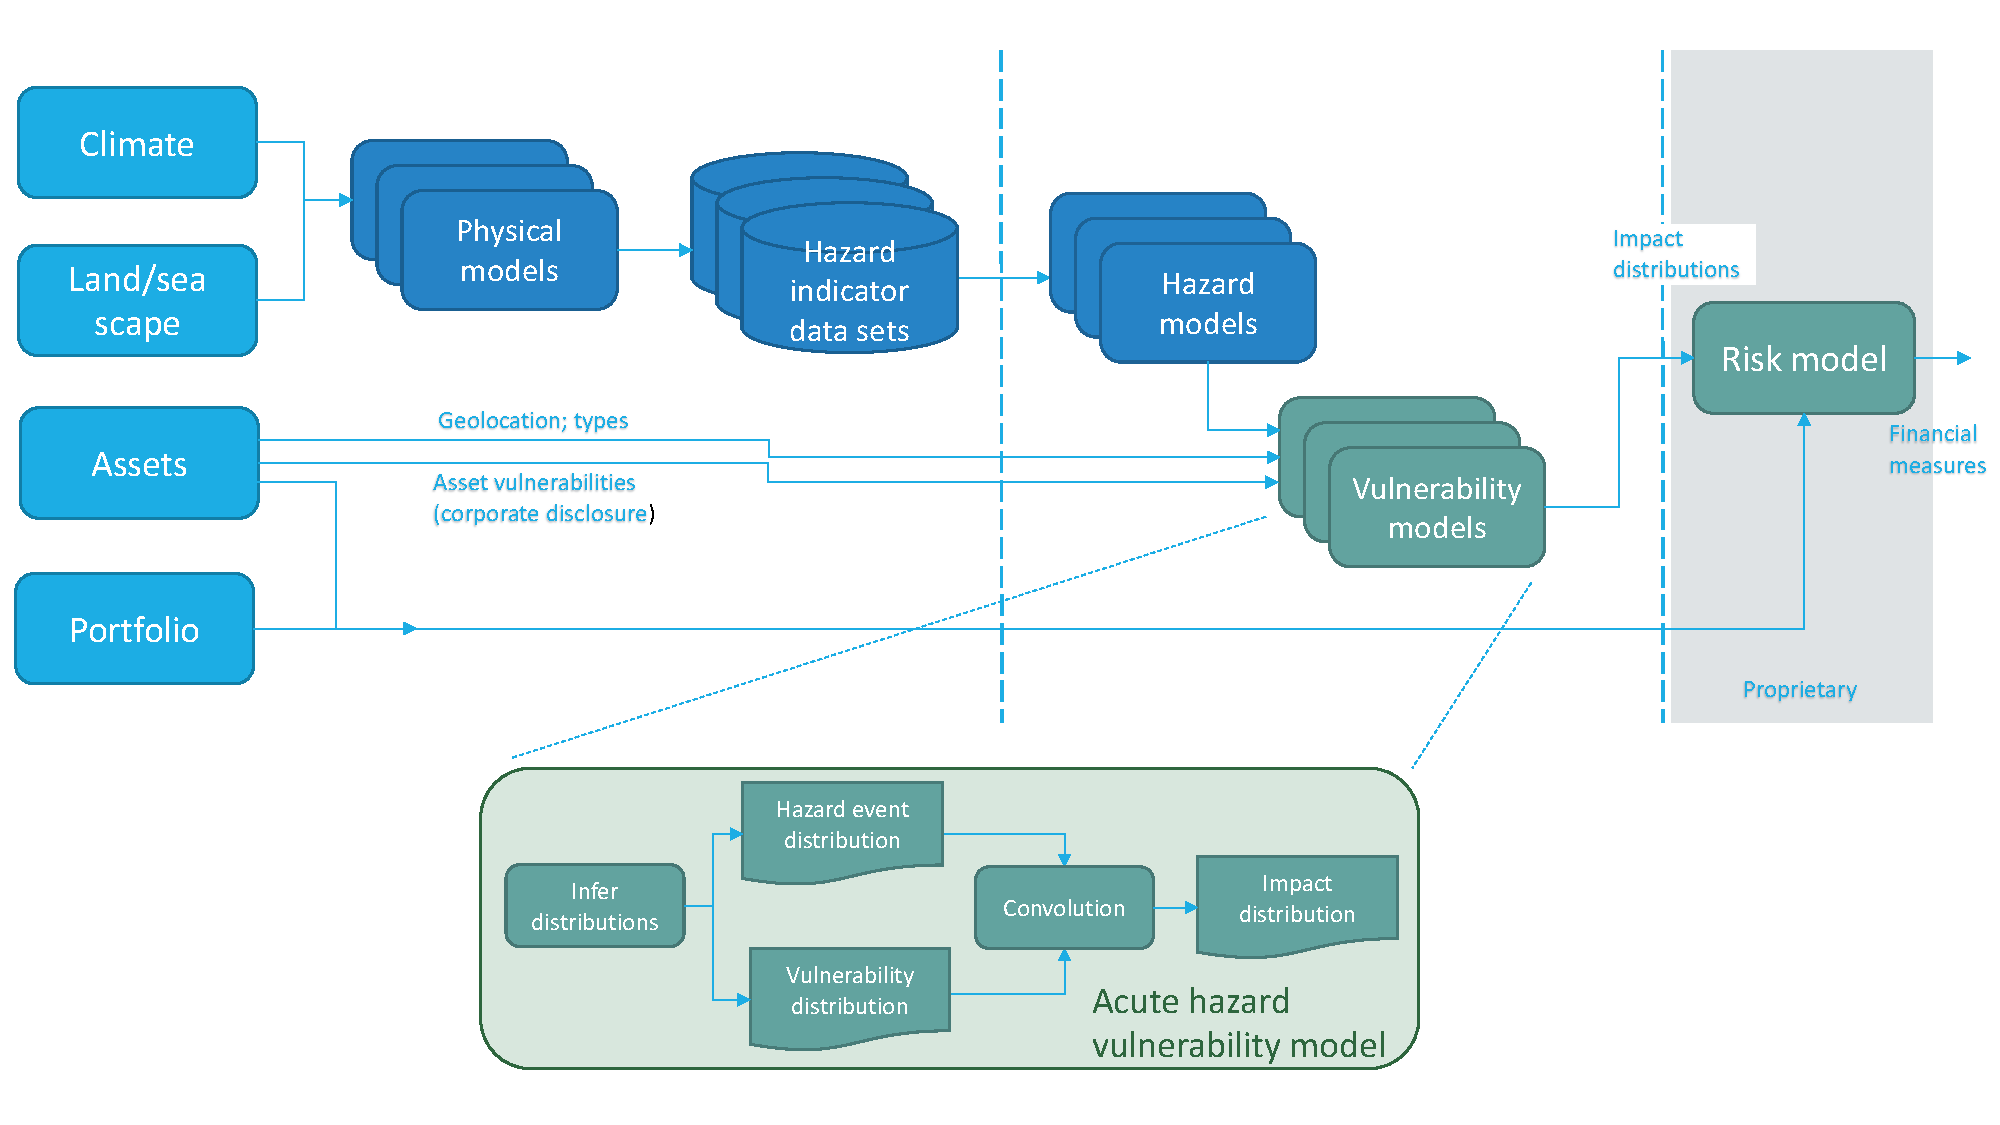
\includegraphics[clip, trim=0cm 0.5cm 0cm 1cm, width=1.00\textwidth]{plots/top_level_view.pdf}

    \end{framed}

    \footnotesize

    \renewcommand{\arraystretch}{1.01}

    \vspace{-3ex}

    \vspace{-0.5ex}

    \caption{\small Physical risk model components. }
    \label{Fig:top_level_view}

\end{figure}
%%%%%%%%%%%%%%%%%%%%%%%%%%%%%%%%%%%%%%%%%%%%%%%%%

\subsection{Hazard model}
As described above, one or more hazard models are used to provide the hazard indicators required by vulnerability models. Vulnerability models request information from hazard models based on location and spatial extent of the assets.

Hazard indicator data sets are available from a number of sources both publicly-available and proprietary. A recent paper \cite{BavandiEtAl:2022} provides a review of sources of the \emph{`forward-looking climate-conditioned hazard data sets'}, as the authors describe the data, that are required by the methodology presented in this document. \cite{RichtersEtAl:2022} provides technical information on the data sets provided by the Network for Greening the Financial System (NGFS) scenarios and provides a useful introduction to scenarios and in particular Representative Concentration Pathways (RCPs) and Shared Socioeconomic Pathways (SSPs) as well as the Coupled Model Intercomparison Project (CMIP) of global climate models data sets. CMIP data sets are very often key inputs into the derivation of forward-looking climate-conditioned hazard indicators.

Subsequent sections include details of both vulnerability models and sources of hazard indicator data sets for each type of hazard. 

\subsection{Vulnerability model}
\label{SubSec:VulnerabilityModel}
The \emph{vulnerability model} determines how an asset is impacted by a hazard. The impact is a quantity from which financial loss can be inferred, but is not itself a monetary value. For example, an impact might be the damage sustained to a building as a fraction of its value or the annual loss of energy output of a power station as a fraction of its annual output\footnote{A systemic change in annual output changes asset value, since this is partly determined by the expected future cash flows generated by the asset.}. In each case, a further (financial) model is required to translate the impact to a change in asset value and thereby a change in financial measure. In principle an impact might lead to an increase or decrease in value.

Catastrophe models sometimes define a quantity `damage', and talk about `damageability'. `Damage' and `impact' are analagous quantities here but `impact' is perhaps better-suited to situations where there is, say, a decrease in output efficiency of a plant as a result of a period of higher temperatures.

Vulnerability models as used in physical risk calculations may overlap with those of catastrophe models. OS-C aims to support a wide range of models, but it is desirable to identify approaches that generalize a large class of these. One such approach is adopted from Oasis LMF \cite{OasisLMF}. The first assumption behind this is that a model should capture two important types of uncertainty, doing so by representing each by a probability distributions:
\begin{enumerate}
    \item Uncertainty as to the frequency and intensity (or severity) of events that potentially lead to a change in asset value. This is sometimes called the {\it primary uncertainty}
    \item Uncertainty as to the vulnerability of assets to events (i.e. response of assets to events of a given intensity), the {\it secondary uncertainty}
\end{enumerate}

These quantities are defined more precisely in \ref{Sec:MathematicalDescriptionOfAssetImpactModel}. Impact can be modelled using a {\it mean impact curve} (or {\it mean damage curve} in catastrophe modelling nomenclature). This is a curve relating an event intensity to an impact (e.g. a wind event with a given maximum gust speed will cause a given fractional damage to a property). In general, however, there is uncertainty as to the impact on an asset to an event of a given intensity -- in the example, the wind may cause mild or severe damage. For this reason, the vulnerability is represented rather as a two dimensional function.

A second assumption is that the probabilities of such events may not be readily represented by distributions such as beta, gamma, beta-Bernoulli or truncated Gaussian and may be complex and multi-modal. Discrete probability distributions are therefore used in order to represent the range of possible distributions: a non-parametric approach. In the mathematical description below, the continuous form of the model is first given followed by a discretisation intended for the capture of non-parametric distributions.

\subsubsection{Mathematical description of vulnerability models}
The output of the vulnerability model is an impact, $d$ for an asset and for a given year\footnote{$d$ for `damage/disruption' is used to denote impact as $i$ is reserved for indexing.}. Physical climate risk analyses are generally concerned with how impacts change as a result of changes to the climate. In contrast with catastrophe modelling where an impact is typically calculated according to a historical baseline, a climate risk calculation would typically compare the baseline to an impact calculated under a particular climate scenario and period in the future.

The impact of hazards on a portfolio of $n$ assets is a (multivariate) probability distribution as a result of the primary and secondary uncertainties. The impact in a given year on a single asset is a random variable, $D$, with (marginal) probability density function $f_D(d)$. The probability of an impact exceeeding $d$ (the \emph{exceedance probability}), $F'_D(d) = \mathbb{P}[D > d]$ is given by:

 \begin{equation}
 	\label{Eq:ImpactExceed}
 	F'_D(d) = \int_d^{\infty} f_D(u) du
 \end{equation}

This is related to the cumulative probability $F_{D}(d) = \mathbb{P}[D \le d]$ by $F'_D(d) = 1 - F_D(d)$. Exceedance probabilities are a popular measure in catastrophe model and the use of $F$ for cumulative probability and $F'$ for exceedance probability will be used hereafter to avoid confusion.

The value of a hazard indicator, which quantifies the intensity of the phenomenon to which the hazard refers (we also use the term `hazard intensity') is given by random variable $S$. This has marginal  probability density $f_S(s)$. This is the probability density of an event occurring in a given year with intensity $s$. This distribution captures the primary uncertainty.

We define a conditional probability density function $f_{D|S}(d, s)$ to be the probability that given the occurrence of a hazard indicator $s$, an impact occurs of size $d$. This distribution captures the secondary uncertainty.

The impact distribution is then given by: 
 
  \begin{equation}
 	\label{Eq:ImpactEffective}
 	f_D(d) = \int_{-\infty}^{\infty} f_S(s) f_{D|S}(d, s) ds
 \end{equation}

Note that $f_d(d)$ is identical to the {\it effective damageability} distribution of Oasis LMF\cite{OasisFinancialModule} and can be described as the `effective impact'. It is a marginal distribution and as such does not capture any correlation between events nor impacts. In the catastrophe models of Oasis LMF, impacts are sampled from this distribution \cite{OasisFinancialModule}, for example samples of fractional damage, which form the basis of a Monte Carlo calculation. This is done in order to apply insurance policy terms and conditions which can be complex and non-linear.

In the case of $n$ assets, multivariate random variables are defined $\mathbf{D} = (D_1,\ldots,D_d)$ and $\mathbf{S} = (S_1,\ldots,S_n)$. We henceforth use the single-asset index $i$ to denote marginal distributions: $f_{S_i}(s_i)$. 

\subsubsection{Return-period-based approach}

The \emph{return-period-based approach} -- sometimes called, a hazard-map-based approach -- makes use of marginal distributions $f_{S_i}$ for each (asset) location $i$, and not the joint distribution, $f_S(\mathbf{s})$. By definition, the marginals are related to the joint distribution by: 

 \begin{equation}
	\label{Eq:ImpactMarginal}
	f_{S_i}(s_i) = \int_{-\infty}^{\infty} \int_{-\infty}^{\infty} \dots \int_{-\infty}^{\infty} f_S(s_1,s_2, \dots,s_n) \,ds_1 \dots ds_{i-1} ds_{i + 1} \dots ds_n
\end{equation}

$f_{S_i}(s_i)$ is usually inferred from a type of hazard indicator data set which are known as \emph{hazard maps}.

\paragraph{Hazard maps.} Hazard maps are three-dimensional data sets from which intensities of hazard indicators can be looked up for different locations and different return periods, i.e. $H(x, y, \tau)$ provides hazard indicator intensity at location $(x, y)$ for return period $\tau$. That is, $H$ is the hazard indicator intensity such that the average time between events with intensity higher than $H$ is $\tau$. 

In order to use hazard maps to derive probabilities, we must, strictly, specify the model of probability of occurrence of events with intensity higher than $H$ assumed by the data set. Occurrence may be modelled by a Poisson distribution as in Equation~\ref{Eq:Poisson}. This gives the probability of $k$ occurrences in time interval $t$ where $\tau$ is the return period.

 \begin{equation}
	\label{Eq:Poisson}
	\mathbb{P}[X = k] = \frac{(t / \tau)^k}{k!}  e^{-\frac{t}{\tau}}
\end{equation}

Alternatively, the number of occurrences can be modelled as a Binomial distribution as in Equation~\ref{Eq:Binomial}, which provides the probability that $k$ occurrences occur in $n$ years, assuming that $\tau$ is specified in years.  

According to Equation~\ref{Eq:Binomial}, \emph{the probability that in a single year there is at least one event with intensity of $H$ or higher is $1/\tau$}. Unless otherwise specified, this is the interpretation used for $\tau$. Note that for Equation~\ref{Eq:Poisson} this relationship only applies approximately.

 \begin{equation}
	\label{Eq:Binomial}
	\mathbb{P}[X = k] = \binom{n}{k} (1/\tau)^k (1-1/\tau)^{n - k}
\end{equation}

$F_{S_i}$ can then be inferred from the hazard map for point-like assets. The curve $H(x_i, y_i, \tau)$ is looked up, providing $\tau$ and thereby annual exceedance probabilities for different intensities, $H$. In the case of a point-like asset, the look up is from spatial coordinates ($x_i$, $y_i$). A hazard map will have an associated co-ordinate reference system (CRS). For example the CRS of whole-globe maps is often the WGS84 World Geodetic System (EPSG:4326). In this case ($x_i$, $y_i$) represent longitude and latitude under that CRS. 

\paragraph{Effective impact.} Once $F_{S_i}$ and thereby $f_{S_i}$ is obtained, Equation~\ref{Eq:ImpactEffective} can be applied to obtain the impact distributions for each location $i$:

 \begin{equation}
	\label{Eq:ImpactMarginal2}
	f_{D_i}(d_i) = \int_{-\infty}^{\infty} f_{S_i}(s_i) f_{D_i|S_i}(d_i, s_i) ds_i
\end{equation}

 In order to aggregate impacts over a portfolio, the dependency structure must be provided; in general, such a dependency structure is specified by a copula\cite{Nelsen:2007}. This may be derived via a heuristic; for example a `worst case' dependency structure could be provided to obtain an upper bound, perhaps assuming 100\% correlation between impacts. In general the approach approach in this section is not intended for cases where accurate treatment of the dependence between the impacts is needed, but rather for:

\begin{itemize}
\item analyses of single assets,
\item quick calculations intended to give an upper bound of an impact, perhaps to identify areas of particular risk, or
\item certain calculations where intra-asset correlation is not required, e.g. expected total ground-up loss.
\end{itemize}

The Sklar theorem of copula theory states that for $n$ random variables~$(D_1, \dots, D_n)$ with joint cumulative density function~(CDF)~$F_D(d_1, \dots, d_n) = \mathbb{P}[D_1 \le d_1, \dots, D_n \le d_n]$, there exists a copula~\mbox{$C:[0,1]^n \rightarrow [0,1]$} such that
\begin{equation}
	\label{Eq:Copula}
	F_D(d_1, \dots, d_n) = C \left( F_{D_1}(d_1), \dots, F_{D_n}(x_n) \right).
\end{equation}
As a reminder, $F_{D_i}(d_i) = \mathbb{P}[D_i \le d_i]$ is the marginal distribution of random variable~$D_i$, \mbox{$i=1, \dots, n$}.

In the general case, Monte Carlo approaches can be used to sample from $F_D$. The approach is:

\begin{enumerate}[]
	\item Sample vector $\mathbf{u}$ from $C$;
	\item Calculate samples for vector $\mathbf{d}$ using the relationship $d_i = F_{D_i}^{-1}(u_i)$.
\end{enumerate}

The samples can then be used to construct a total damage, for example, via $\sum_i d_i$.

Under heuristic approaches a Gaussian copula might be chosen:
\begin{equation}
	\label{Eq:CopulaGaussian}
	C^{\text{Gaussian}}_K(\mathbf{u}) = \Phi_n(\Phi^{-1}(u_1), \dots, \Phi^{-1}(u_n);\mathbf{K}),
\end{equation}
where $\Phi(z)$ is the CDF of a standard normal variable, and $\Phi_n(\mathbf{z}; \mathbf{K})$ denotes a joint standard normal multivariate~CDF with mean zero and correlation matrix $\mathbf{K}$. Samples $\mathbf{u}$ can be obtained by the approach:

\begin{enumerate}[]
	\item Sample vector $\mathbf{z}$ of correlated normal random numbers,
	\item Calculate samples for vector $\mathbf{u}$ using the relationship $u_i = \Phi_i(z_i)$.
\end{enumerate}

As an example, if impact distributions represent damage to buildings as a result of inundation then one may attempt to model damage to two buildings in close proximity as being highly correlated. However catastrophe model practitioners might point out that even such considerations as the presence or absence of kerb stones and availability of sand bags are highly significant so any such assumption is prone to error. If the buildings are far apart (say in different continents) then the correlation is likely to be close to zero however. The two extremes of 0\% and 100\% correlation of impacts are special cases of this general approach and it may be appropriate to run calculations with such cases to obtain an estimate of the impact of correlation -- rather than to attempt to model correlation more precisely. 


\subsubsection{Event-based approach}
As mentioned in the previous section, where an accurate treatment of the dependence between impacts is needed, a heuristic is unlikely to be adequate. This can occur, for example, where it is required to model the occurrence of a 1 in 250 years `worst-case' event, the event being `worst-case' for a specific portfolio\footnote{In general, a `1 in 250 year' event for a portfolio is an ambiguous statement and requires the definition of a measure. For example the `1 in 250 year' \emph{ground-up loss} of a portfolio is unambiguous. For a single asset, `1 in 250 year' is unambiguous if impact is assumed to be a non-decreasing function of hazard intensity.}. In such cases, it is necessary to model the dependence of hazard intensity and vulnerability explicitly. In an event-based approach, this is achieved by calculating the impact of a large number of events. An event might, for example, be a flood or storm affecting a particular geographical region. Events can be:

\begin{itemize}
	\item historical events, or
	\item synthetic, `plausible' events.
\end{itemize}

In the case of synthetic events, the event may itself be probabilistic; at a particular time, in a particular part of the region, the intensity of the hazard might be represented by a probability distribution. However historical events are typically deterministic and synthetic event sets are often deterministic also; unless otherwise stated, this will be assumed to be the case.

\paragraph{Relationship to hazard maps.}
Events may be specified with respect to hazard maps; that is the hazard data comprises both hazard map and event set. Typically in such cases the severity of an event is specified using a return period which can then be related back to the hazard map.

More formally, for each event, index $j$, a function $z_j$ is defined such that $\tau_{i, j} = z_j(x_i, y_i)$. Here $\tau_{i, j}$ is the severity of the event specified as a return period for asset index $i$ and event index $j$.  $(x_i, y_i)$ are the coordinates of the asset in the relevant CRS.

For the given event, $\tau_{i, j}$ is then used to look up a hazard intensity, from the hazard map:
 
 \begin{equation}
	\label{Eq:Severity1}
	s_{i, j} = H(x_i, y_i, \tau_{i, j}) 
\end{equation}

Note that here $s_{i, j}$ is deterministic \emph{for a given event} and we have simply for the impact distribution for event $j$:

 \begin{equation}
	\label{Eq:Severity2}
	f_{D_i, j}(d_i) = f_{D_i|S_i}(d_i, s_{i, j})
\end{equation}

For each event and each asset, we can then draw $m$ samples from $f_{D_i, j}(d_i)$. The samples across all assets for a single event are drawn jointly using a copula as per Equation~\ref{Eq:Copula} to capture the dependence structure of impacts. Such an approach can be important if levels of damage sustained under a given hazard intensity are correlated between assets, which might be the case if the assets are similar in construction. However, by default samples are assumed to be independent. That is the approach is:

For each of $n$ events, and for each of $m$ samples:
\begin{enumerate}[]
	\item sample vector $\mathbf{u}$ of uncorrelated random numbers $\mathbf{U} \stackrel{iid}{\sim} U[0, 1]$;
	\item calculate vector $\mathbf{d}$ using the relationship $d_i = F_{D_i, j}^{-1}(u_i)$.
\end{enumerate}

The resulting $n \times m$ sets of impacts for the portfolio of assets is the inputs into the financial model.

\paragraph{Constant severity regions}
Under a constant severity region approximation, $\tau_{i, j}$ is a constant across each asset $i$ for a particular event $j$.
 

\subsubsection{Discrete form of acute vulnerability model}
\label{Sec:MathematicalDescriptionOfAssetImpactModel}

The continuous forms of expressions for the impact distribution are given by Equation~\ref{Eq:ImpactMarginal2} and Equation~\ref{Eq:Severity2}, the latter being the special case of deterministic hazard -- generally encountered for one specific event. Here a discrete version of Equation~\ref{Eq:ImpactMarginal2} is defined.

There are $n_h$ intensity bins with index $q$ such that $q \in \{1, \dots, n_h \}$.  $\sigma^{(h)}_q$ is defined to be the probability that a hazard event of type $h$ occurs in a given year with an intensity that falls in bin $q$. With random variable $S^{(h)}$, now with superscript, being the intensity of hazard type $h$:

\begin{equation}
    \label{Eq:Discrete1}
    \sigma^{(h)}_q = \mathbb{P} \left[ s^{(h, \text{lower})}_q < S^{(h)} \le s^{(h, \text{upper})}_q \right]
\end{equation}

That is, $s^{(h, \text{lower})}_q$ and $s^{(h, \text{upper})}_q$ define the range of bin $q$. For the avoidance of doubt, $\sigma^{(h)}_q$ is related to the continuous probability density $f_S(s)$ by:

\begin{equation}
	\label{Eq:Discrete2}
	\sigma^{(h)}_q = \int_ {s^{(h, \text{lower})}_q}^{s^{(h, \text{upper})}_q} f_S(s) ds 
\end{equation}

We define $v^{(h, b)}_{pq}$ to be the conditional probability that \emph{given} the occurrence of an event associated with a hazard of type $h$ and with intensity $s^{(h)} \in (s^{(h, \text{lower})}_q, s^{(h, \text{upper})}_q]$ there is an impact of type $b$, $d^{(b)} \in (d^{(b,\text{lower})}_p, d^{(b,\text{upper})}_p]$. $b$ may be, for example, damage incurred expressed as a fraction of the asset present value. 


\begin{equation}
    \label{Eq:vulnerability}
    v^{(h, b)}_{pq} = \mathbb{P} \left[ d^{(b,\text{lower})}_p < D^{(b)} \le d^{(b,\text{upper})}_p | s^{(h, \text{lower})}_q < S^{(h)} \le s^{(h, \text{upper})}_q \right]
\end{equation}

The definition of an event type $h$ includes a time interval e.g. $h$ is the occurrence of an inundation in the locale of the asset {\it within a one year period}. $b$ is, for example, the fractional damage to the asset.

$\delta^{(h,b)}_p$ is defined to be the marginal probability of impact $D^{(h, b)}$ in the range $d^{(b, \text{lower})}_p < D^{(h, b)} \le d^{(b,\text{upper})}_p$ occurring as a result of an event of type $h$.

\begin{equation}
    \label{Eq:impact}
    \delta^{(h, b)}_p =  \mathbb{P} \left[ d^{(b,\text{lower})}_p < D^{(h, b)} \le d^{(b,\text{upper})}_p \right]
\end{equation}

From the definition of conditional probability:

\begin{equation}
    \label{Eq:model}
    \delta^{(b)}_p = \sum_{q} v^{(h,b)}_{pq} \sigma^{(h)}_q
\end{equation}

If only the mean impact curve is available, then it is possible to create the matrix such that $v_{pq} \in \{0, 1\}$. The matrix then provides a simple mapping from intensity to impact; if the number of intensity and response bins is equal then matrix $\mathbf{v}$ is simply the identity matrix. However, note that these simplifications exclude from the model any uncertainty in the parameters\footnote{A better approach would be to estimate the standard deviation of the distributions from which the mean impact curve was calculated and to incorporate this.}.

\paragraph{Multiple occurrence of events.} Note that $\sigma^{(h)}_q$ is the probability of occurrence of \emph{at least one event} with intensity in bin $q$ in a year and the vulnerability, $v_{pq}$ gives the probability of impact given at least one event has occurred. Some care must therefore be taken when using probabilities $v_{pq}$ calibrated from single events as there is an implied approximation that either probability of multiple events is small and/or that impact is well-modelled as a single impact from the most intense event for a given year. 


\subsubsection{Importance of secondary uncertainty}

%%%%%%%%%%%%%%%%%%%%%%%%%%%%%%%%%%%%%%%%%%%%%%%%%
\begin{figure}[ht]
	
	\begin{framed}
		
		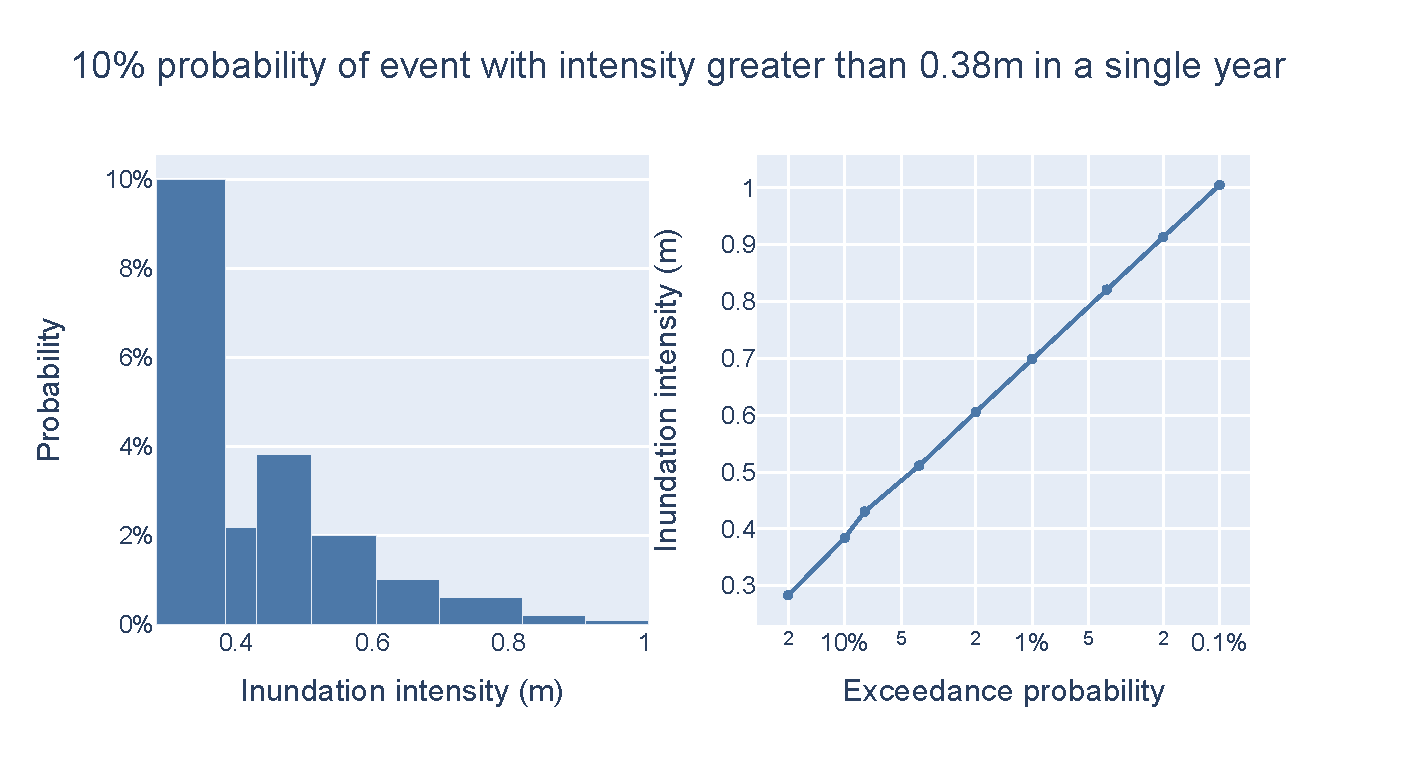
\includegraphics[width=\textwidth]{plots/fig_intensity.pdf}
		
	\end{framed}
	
	\footnotesize
	
	\renewcommand{\arraystretch}{1.01}
	
	\vspace{-3ex}
	
	{\justify
		The exceedance curve of event intensity at the asset location is shown on the right. The event intensity in this example is inundation depth in metres. Exceedance is a cumulative probability. As an example, the probability of an inundation event occurring within a single year of intensity 0.91m or greater is 0.2\%. An exceedance probability is the reciprocal of the return period; it could equivalently be said that the 0.91m intensity event occurs with a return period of 500 years.
		The exceedance curve can be converted to a histogram of probabilities. Here the $n_h$ bins have ranges $(s^{(h, \text{lower})}_q, s^{(h, \text{upper})}_q]$. For example, the first bin has range (0.28m, 0.38m]. The second bin has range (0.38m,    0.43m]; that is $s^{(h, \text{lower})}_2 = 0.38$m and $s^{(h, \text{upper})}_2 = 0.43$m. $\sigma^{(h)}_2 = 0.02$.
		\par}
	
	\vspace{-0.5ex}
	
	\caption{\small Event intensity exceedance curve (right) and corresponding histogram (left).}
	\label{Fig:intensity}
	
\end{figure}
%%%%%%%%%%%%%%%%%%%%%%%%%%%%%%%%%%%%%%%%%%%%%%%%%


The importance of the vulnerability matrix as opposed to mean damage curve (or vector) is emphasized above; see also \cite{Taylor:2015} for a discussion of this point. This is true not only in cases where the underlying distribution of an impact, for example a fractional damage, can be inferred from empirical data; see for example Figure~\ref{Fig:vulnerability_matrix}. This is arguably \emph{more} important where data is limited in order that approximate data can be incorporated into the model in a way that the impact of the approximations can be well-understood.

Vulnerability data may be provided by
\begin{itemize}
    \item modelling of asset vulnerability based on asset characteristics and/or historical data, or
    \item 'calibrated' vulnerabilities, for example based on realized insurance claims
\end{itemize}
Physical risk models may make use of so-called `bulk assessment' approaches for certain assets, where precise vulnerability information is not available and less precise estimates of the damage/disruption of the asset are used. The presence of such estimates in an overall model may, or may not, materially impact the accuracy of the results, but it is important that this impact can be assessed. By quantifying the uncertainty in the response estimates, a distribution of financial losses is ultimately obtained from which the model user can derive the impact of the approximation.

\paragraph{Including epistemic uncertainty in vulnerability.}
In forms of bulk-assessment, and indeed in other cases, a common occurrence is that insufficient information exists with which to characterize an asset. This is an example of an epistemic, as opposed to aleatory, uncertainty. The epistemic uncertainty, and its impact, can be included in the model in the following way.

We extend Equation~\ref{Eq:vulnerability}, by including a new discrete random variable, $A$, which is an integer index, $A \in \{0, ..., n_a\}$, indicating the type of the asset. We define $v^{(h, b)}_{pqa}$ to be the probability that $D^{(h, b)} \in (d^{(b,\text{lower})}_p, d^{(b,\text{upper})}_p]$ given that $S^{(h)} \in (s^{(h, \text{lower})}_q, s^{(h, \text{upper})}_q]$ \emph{and} the asset in question is of type $a$:
\begin{equation}
    \label{Eq:spistemic1}
    v^{(h, b)}_{pqa} = \mathbb{P} \left[ D^{(h, b)} \in (d^{(b,\text{lower})}_p, d^{(b,\text{upper})}_p] | S^{(h)} \in (s^{(h, \text{lower})}_q, s^{(h, \text{upper})}_q], A = a \right]
\end{equation}

The conditional probabilities can then be combined:
\begin{equation}
	\label{Eq:epistemic2}
	v^{(h, b)}_{pq} = \sum_a v^{(h, b)}_{pqa}  \mathbb{P}[A = a]
\end{equation}

$\mathbb{P}[A = a]$ is the \emph{prior} probability that the asset is of type $a$. This may be obtained from knowledge of the make-up of a portfolio.

Note that through the application of Equation~\ref{Eq:model} the impact distribution now depends on the prior probabilities. To illustrate why it is reasonable that this should be the case, say we have two types of assets in our portfolio. Type A is vulnerable to a hazard with an intensity that has a relatively short return period of 50 years, whereas type B is invulnerable to all hazards but those with a vanishing small probability of occurrence. To derive the probability that an asset is damaged by a certain amount in a given year using Equation~\ref{Eq:epistemic2}, we must allow for the possibility that the asset may be of type A and may therefore be damaged as a result of 50 year events.

\paragraph{Epistemic uncertainty as source of error.} An alternate approach is to treat epistemic uncertainty as a source of error rather than, or in addition to, including it in the vulnerability as we have done here. This might be driven by the observation that as information as to the identity of assets is improved then the exceedance probability of a certain impact will change. This can be achieved by running an ensemble of calculations, changing the prior probabilities in each case. 

\subsubsection{Interpolation of probability distributions}
Cases arise where the event distributions and vulnerability distributions are not defined for a common set of intensity bins and interpolation is therefore required. The question then arises of how probability density is distributed within bins. The choice is model-specific and customizable, but here two common cases are described.

\begin{itemize}
    \item Probability density constant across bin: linear interpolation of cumulative probability function
    \item Probability density changes linearly across bin: quadratic interpolation of cumulative probability function
\end{itemize}

{\textcolor{red}{\emph{[Add equations and example plots here]}}}

Hazard data sets might also contain instances of `point-probabilities', for example where there is a finite probability that the intensity of an event takes a single value. These represent Dirac delta functions in the probability distribution, steps in the cumulative probability function. There is the option of retaining these as delta functions (bins of zero width), but in some cases it may be necessary to make assumptions about how these the probability might be distributed across a bin.

{\textcolor{red}{\emph{[Add equations and plot of step-CDF with interpolation; exemplify by `damage threshold']}}}

\subsubsection{Probability bins from hazard maps}

From Equation~\ref{Eq:Discrete2} the probability of an event occurring with hazard intensity in bin $q$ is expressed in terms of the probability density $f_S$ (dropping superscript $h$ for clarity):

\begin{equation}
	\label{Eq:Discrete2Again}
	\sigma_q = \int_ {s^{(\text{lower})}_q}^{s^{(\text{upper})}_q} f_S(u) du \
	= \int_ {s^{(\text{lower})}_q}^{\infty} f_S(u) du - \int_ {s^{(\text{upper})}_q}^{\infty} f_S(u) du
\end{equation}

The exceedance probability $F_S'$ is defined as:

\begin{equation}
	\label{Eq:DiscreteExceed}
	F'_S(s) = \int_s^{\infty} f_S(u) du
\end{equation}

from which we can write:

\begin{equation}
	\label{Eq:DiscreteExceed2}
	\sigma_q = F'_S({s^{(\text{lower})}_q}) - F'_S({s^{(\text{upper})}_q})
\end{equation}

Using Equation~\ref{Eq:DiscreteExceed2}, a set of probability bins for the hazard event can be inferred from an exceedance probability curve. An exceedance probability curve can readily be inferred from a return-period curve using the result that the annual exceedance probability is the reciprocal of the return period expressed in years.

As an example, suppose that we have a hazard map for flood which contains return periods of 2, 5, 10, 25, 50, 100, 250, 500 and 1000 years. For a certain latitude/longitude the flood depths corresponding to the 9 return periods are, in metres: 0.06, 0.33, 0.51, 0.72, 0.86, 1.00, 1.15, 1.16 and 1.16. The data is shown together with the exceedance probability in Table~\ref{Table:HazardData}. 

\begin{table}[ht]
	\caption{Example hazard event data.} 
	\centering 
	\begin{tabular}{c c c c} 
		\hline
		Return period (years) & Flood depth (m) & Exceedance probability  \\ [0.5ex] 
		\hline 
		2 & 0.06 & 0.5 \\
		5 & 0.33 & 0.2 \\ 
		10 & 0.51 & 0.1 \\ 
		25 & 0.72 & 0.04 \\ 
		50 & 0.86 & 0.02 \\ 
		100 & 1.00 & 0.01 \\ 
		250 & 1.15 & 0.004 \\ 
		500 & 1.16 & 0.002 \\ 
		1000 & 1.16 & 0.001 \\ 
		\hline 
	\end{tabular}
	\label{Table:HazardData} 
\end{table}

The flood depths become the bin edges of the probability distribution and the probabilities are calculated from Equation~\ref{Eq:DiscreteExceed2}. For example, the probability of occurrence of a flood with depth in the range (0.86m,  1.00m] is $0.02 - 0.01 = 0.01$\footnote{Care is needed at either end of the curve. There is a 0.001 probability that flood depth exceeds 1.16m in this example; should this be included in the (point-like) 1.16m bin?}. Note that in defining a set of bins in this way, no assumption about the interpolation between the flood depths is required. However, if we assume this to be linear then this implies that the probability density is constant across each bin since $f_S = \frac{dF_S(s)}{ds}$.


\subsubsection{Vulnerability distributions and heuristics}
For some assets, a vulnerability matrix may be available, corresponding to the `ideal' case  of Figure~\ref{Fig:vulnerability_matrix}. That is, for each intensity value a probability distribution of the impact (damage/disruption) is given. In other cases, only the impact itself is available for a given hazard intensity -- a damage curve -- together with some measure of uncertainty. Here the probability distribution is unknown, but it is at least possible to fit some choice of distribution to the descriptive statistics (e.g. mean and standard deviation).

Given that the distribution of fractional impact -- e.g. damage  as a fraction of asset value or disruption as a fraction of output capacity -- is in the range  (0, 1), heuristic choices of distributions include Beta and Truncated Gaussian \cite{MitchellEtAl:2017}. It should be emphasized that neither distribution is likely to be correct, especially in lacking multi-modality and fat-tails, but provide a method by which uncertainty in the impact can be taken into account.

\paragraph{Modelling impact using a Beta distribution.}
The cumulative probability function of a Beta distribution is given by:

\begin{equation}
	\label{Eq:Beta1}
	F_{\text{Beta}}(x) = \frac{B(x; a, b)}{B(1; a, b)} ,
\end{equation}

where $0 < x < 1$ and $B(x; a, b)$ is the incomplete Beta function:

\begin{equation}
	\label{Eq:IncompleteBeta}
	B(x; a, b) = \int_0^{x} t^{a-1} (1 - t)^{b-1} dt .
\end{equation}

If the mean, $\mu$ and standard deviation, $\sigma$ of the impact distribution are known then \cite{MitchellEtAl:2017}:

\begin{equation}
	\label{Eq:BetaA}
	a = \frac{(1 - \mu)}{c^2} - \mu ,
\end{equation}

\begin{equation}
	\label{Eq:BetaB}
	b = \frac{a(1 - \mu)}{\mu}
\end{equation}

where

\begin{equation}
	\label{Eq:BetaC}
	c = \frac{\sigma}{\mu}
\end{equation}

In order to calculate the impact, the set of bins $p$ that define the impact probabilities $\delta_p$ of interest are first defined. The vulnerability matrix $v_{pq}$ of Equation~\ref{Eq:vulnerability} is then calculated. In order to apply Equation~\ref{Eq:Beta1}, $a$ and $b$ are calculated using mean and standard deviations of impact calculated at the mid-point of each intensity bin. We then have:

\begin{equation}
	\label{Eq:BetaVuln}
	v_{pq} = F_{\text{Beta}}(d_p^{(\text{upper})}; a_q, b_q) - F_{\text{Beta}}(d_p^{(\text{lower})}; a_q, b_q)
\end{equation}

$a_q$ and $b_q$ are the values of $a$ and $b$ calculated from means and standard deviations calculated at the intensity bin centre $s_q = \frac{s_q^{(lower)} + s_q^{(upper)}}{2}$.

%%%%%%%%%%%%%%%%%%%%%%%%%%%%%%%%%%%%%%%%%%%%%%%%%
\begin{figure}[ht]

    \begin{framed}

		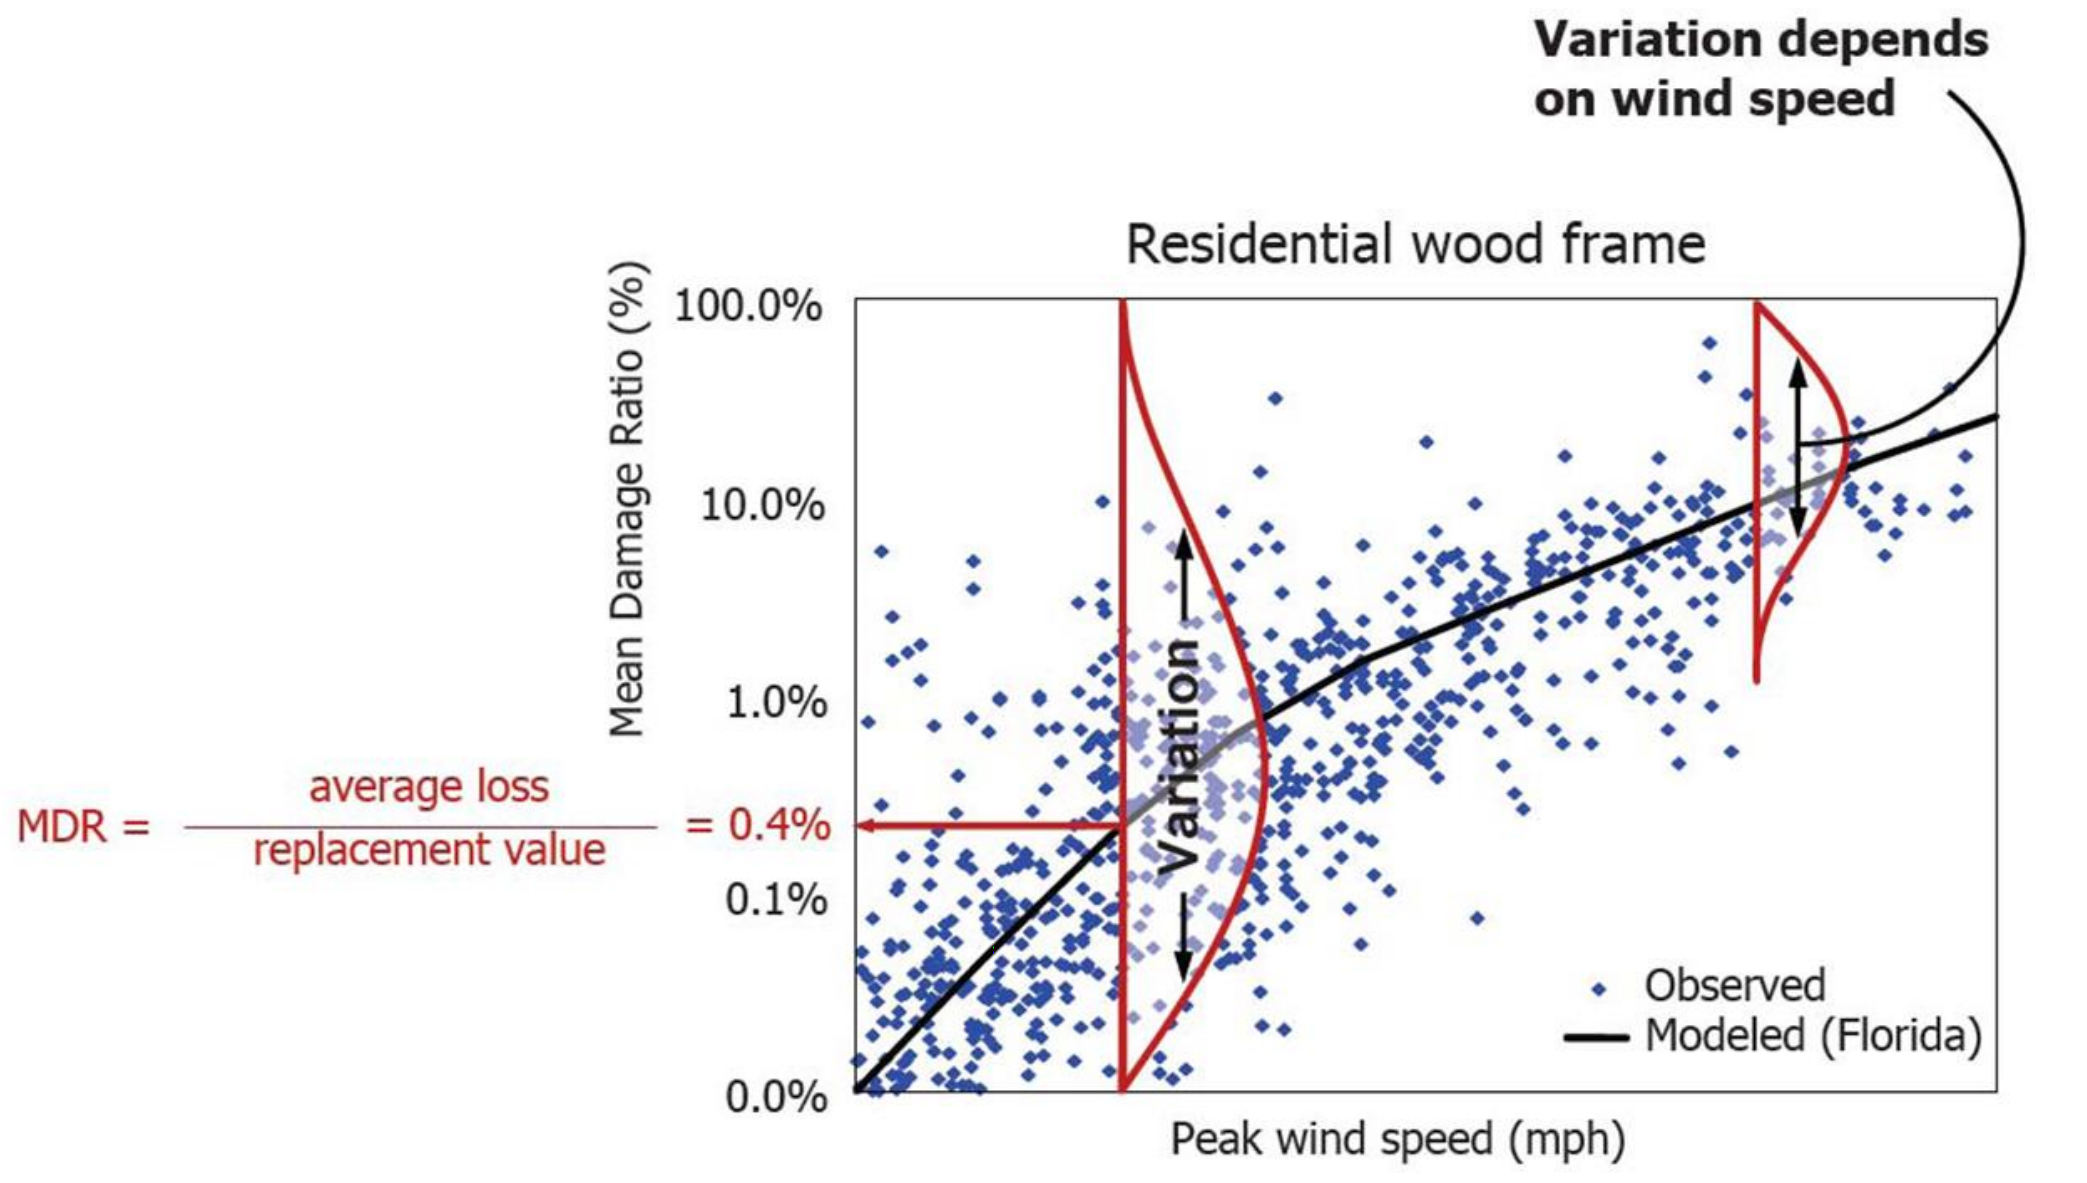
\includegraphics[width=\textwidth]{plots/vulnerability_lagace_2008.png}

    \end{framed}

    \footnotesize

    \renewcommand{\arraystretch}{1.01}

    \vspace{-3ex}

%    {\justify
%        Taken from
%        \par}

    \vspace{-0.5ex}

    \caption{\small Taken from Lagacé (2008) Catastrophe Modeling, Université Laval. Mean damage curve as an approximation to an underlying set of distributions, modelled using a vulnerability matrix.}
    \label{Fig:vulnerability_matrix}

\end{figure}
%%%%%%%%%%%%%%%%%%%%%%%%%%%%%%%%%%%%%%%%%%%%%%%%%


\subsection{Aggregation of impacts}
For impacts of the same type, $b$, arising from different events, it is assumed that the impacts are additive, up to a ceiling value\footnote{this approximation is only strictly valid for sufficiently small impacts; consider the contrived example of 0.8 fractional damage that occurs from both flood and high wind in the same year.}. If the annual impacts from events with index 1 and 2 are represented by random variables, $Y^{(1,b)}$, $Y^{(2,b)}$ then $Y^{(\text{tot}, b)} = Y^{(1,b)} + Y^{(2,b)}$.

If the random variables are uncorrelated, then the aggregated effective impact distribution is given by the convolution:

\begin{equation}
    \label{Eq:sampling}
    y^{(\text{tot}, b)}(r) = \int^{\infty}_{-\infty} y^{(1, b)}(t) y^{(2, b)}(r - t) dt
\end{equation}

{\textcolor{red}{\emph{[Add version with discrete binned data.]}}}

\subsection{Financial model}

\subsubsection{Types of calculation.}
Vulnerability models were described in \ref{SubSec:VulnerabilityModel} as a means to calculate the damage and disruption to a portfolio of assets for different hazard models. How the resulting probability distributions of impact are then used in a financial model depends on the intent of the analysis. We distinguish between \emph{stress test} and \emph{portfolio analysis} use cases. 

\emph{Stress tests} make use of climate-related shocks -- severe acute events -- in order to assess an impact. This might for example be the impact on a financial institution. Stress tests may make use of narrative scenarios or may take the approach of simulating large number of extreme but plausible events in order to identify a worst-case which is \emph{a priori} unknown. Indeed the two approaches may be combined, assessing the impact of a severe acute event coupled with other aggravating factors.

In a \emph{portfolio analysis}, the aim is to assess which parts of a portfolio of assets are most subject to physical climate risk. 

\subsubsection{Climate risk measures and importance of change.}
Climate risk models generally differ from catastrophe models in more than their use of climate-conditioned and projected hazard models. In particular, physical climate risk arises from \emph{changes} in climate.

We take as an example a real estate asset that is collateral for a loan. The hypothetical asset is exposed to both hurricane and flood hazards today, however it is covered by an insurance policy and its current valuation takes into account both historical occurrence of hazards and the policy details. Risk managers concerned with climate risk are likely to be interested in potential changes in value of the asset over the full term of the loan:

\begin{enumerate}
	\item if acute events become more frequent and severe, assets may become more expensive to insure and less desirable {\textcolor{red}{\emph{[Citation]}}} \footnote{For example, to a resident of a house subject to regular flooding.}, which can decrease the asset value;
	\item if an extremely severe and widespread event occurs, default may lead to a distressed sale and/or the full insurance payout may not be made. 
\end{enumerate}

For a portfolio analysis, it is therefore likely to be the change in frequency of events and the change in probability of extremely severe events that is particularly of interest; these are the risk drivers.

\paragraph{Definition of measures.} For a portfolio, distributions of annual impacts, typically damage and disruption, can be aggregated and converted into distributions of change in portfolio value in a given reporting currency. Measures describing the loss of value are:

\begin{enumerate}
    \item Annual Exceedance Probability (AEP): the probability that in a given year the aggregated losses of a portfolio will exceed a certain value.
    \item Average Annual Loss (AAL): the mean value of the aggregated losses of a portfolio in a given year.
\end{enumerate}

From the argument above, a change in AEP for moderate and severe loss cases can be a useful indicator of risk. The change is from historical baseline to a climate-conditioned projection.

\subsubsection{Structural models of credit risk}
Changes in asset value can be used to model changes in the credit quality of market participants. Financial risk modules for physical risk may then use distributions of asset value changes in order to model changes of credit quality over time as a result of climate change, for example estimates of default probability and loss given default.

The intention of this section is not to specify any particular model, but rather to give a brief introduction. Particularly of interest is the question of what inputs credit risk models require.

For medium and large cap firms, a credit default event typically occurs when a firm is not able to meet its debt servicing obligations. Under an important class of credit risk models called `structural models', it is assumed that a default event occurs for a firm when its assets are sufficiently low compared to its liabilities.

A number of different structural models exist which make various assumptions about how a firm's assets change over time, how its capital is structured and the nature of its debt.

The earliest structural model was described by Merton in 1974 \cite{Merton:1974} based on an extremely simple debt structure. Black and Cox \cite{BlackCox:1976} introduced an important refinement to the Merton model in 1976. Practical implementations were subsequently created as a result of this foundational work. A notable one of these is the `KMV' model, named after Kealhofer, McQuown and Vasiek, now owned by Moody's Investors Service, Inc.

Use of such credit models, may provide a mechanism for incorporation of physical risk into financial institutions existing risk models\cite{KenyonEtAl:2021}.

\subsection{Uncertainties in the calculation}

\subsection{Model limitations}

\begin{enumerate}
    \item Spatial correlation of events: to what extent possible without MC calculation; to what extent is provided / can be inferred from data sets
    \item Correlation of vulnerability
    \item Data availability
\end{enumerate}


\subsubsection{Data availability}
Issues related to data availability and relevance are still one of the main limitations of physical risks assessments. If past and future climate data are becoming increasingly available through open-sources portals and tools (e.g. Copernicus, WRI Aqueduct), their availability and their reliability varies widely according to the climate hazard of interest, the region and the modelling process. If the availability of climate data is improving, open-source, asset-level information (required to estimate the exposure of an asset to a give climate hazard) is still seldom available. Such data include the location of assets, their link with owning companies and more generally any damages records that could be used to quantify the response of an asset (or of a type of asset) to a given climate event. Newly-published datasets have been recently released for some sectors but their exhaustiveness remains to be verified. Moreover, many industrial sectors are not covered, thus limiting the application of physical risks methodologies to a diversified portfolio.
Finally, building and applying the correlation between hazard and damage (or impact), as described in section 2.2, requires common distribution between historical events, historical damages and future climate events. In a changing climate, assets and activities will be impacted by more intense events that will not have been experienced either in a given region of the world or even on the
whole globe, leading to a potentially large mismatch between historical and future distributions of events. The interpolation of the damage curve, as described in section 2.2.3, might lead to very high uncertainties that need to be taken into account when interpreting the data.





%\section{Hazard and vulnerability models}

\section{Inundation}
\subsection{Hazard models}
Inundation is modelled as an acute risk using the approach of Section~\ref{SubSec:AcuteAssetImpactModel}. Hazard event models compatible with this method provide inundation depths for different annual probabilities of occurrence -- or equivalently return periods. The need for sufficient granularity in the set of return periods is discussed in \cite{WardEtAl:2011}. 

Inundation hazards are incorporated into physical risk calculations using the World Resource Institute (WRI) Aqueduct flood model \cite{WardEtAl:2020} which has relatively high return-period granularity. This is based on the global modelling approach of \cite{WardEtAl:2013}.

{\textcolor{red}{\emph{[Discuss and include refs for approaches based on flooded area?]}}}

\subsection{Vulnerability models}
Notable damage models for real estate assets include the FEMA FAST `HAZUS' model \cite{ScawthornEtAl:2006} and an European Commission Joint Research Centre (JRC) model \cite{HuizingaEtAl:2017}. The latter is implemented in the \emph{physrisk} library. 
 

\section{Heat}

Heat is classified as both a chronic and an acute hazard.  For example, increased average temperature in a particular area can lower average productivity from labour or make the area less desirable as a place to live, lowering real estate prices. We classify these as risks from chronic hazards. Heat waves are examples of acute hazard events; a period of particularly high temperature might lead to the complete suspension of industrial activity.

Multiple indexes for quantifying heat hazards have been suggested and multiple approaches for the modelling of acute events are present in the literature, e.g. \cite{MazdiyasniEtAl:2019}. Similarly, various methods for modelling the vulnerability to heat hazards have been suggested. Analyses of heat wave events are commonly based on Global and Regional Circulation Model (GCM and RCM) outputs \cite{DosioEtAl:2018}. In \cite{Christidis:2021} and \cite{Christidis:2013} the authors analyse ensembles of CMIP6 simulations with and without anthropogenic forcings in order to determine if extreme heat events are attributable to (anthropogenic) climate change. Such attribution analysis is based in part on finding return periods of events (see also \cite{StottEtAl:2016}). This estimation of return periods for events is directly applicable to acute hazard models.  

In order to support a wide range of hazard and vulnerability models,  \emph{physrisk} includes the derivation of heat statistics from CMIP6 data\footnote{This is somewhat in contrast to the use of the Aqueduct model of \cite{WardEtAl:2020} for modelling inundation where the complete hazard model is used as-is within \emph{physrisk} -- albeit reformatted to handle efficiently the access patterns needed for physical risk calculations.}. 

\subsection{Hazard Models}

\subsubsection{Chronic hazard models}
As mentioned above, hazard models and vulnerability models are closely coupled. \cite{ZhangAndShindell:2021} describes the `GZN' (Graff-Zivin and Neidell) and `WBGT' (WetBulb Globe Temperature methodology) methods. The statistics required for these methods are derived using bias-corrected and down-scaled data sets. There are multiple sources of data suitable for the estimation of the required statistics, notably the NEX-GDDP-NASA set \cite{ThrasherEtAl:2022}.



\subsubsection{Acute hazard models}
Acute hazard modelling approaches are based on calculating return periods of events in a way analogous to acute inundation models. The calculation of return periods from data sets presents a statistical challenge, dealt with for example by \cite{MentaschiEtAl:2016}.



%%%%%%%%%%%%%%%%%%%%%%%%%%%%%%%%%%%%%%%%%%%%%%%%%%%%%%%%%%%%%%%%%%%%%%%%%%%%%%%%%%%%
%%%%%%%%%%%%%%%%%%%%% Changes - Heat Vulnerability Model %%%%%%%%%%%%%%%%%%%%%
%%%%%%%%%%%%%%%%%%%%%%%%%%%%%%%%%%%%%%%%%%%%%%%%%%%%%%%%%%%%%%%%%%%%%%%%%%%%%%%%%%%%


\subsection{Heat Vulnerability Model}

\label{SubSec:HeatVulnerabilityModel}

\subsubsection{Impact of Temperature on labour productivity}

The Heat vulnerability model presented in this section is based on the approach introduced in 'Temperature And Work: Time allocated to work under varying climate and labor market conditions' (2021)\cite{TemperatureAndWork:2021}. The paper uses survey data to estimate labour allocation decisions in the United States (US) based on temperature. It does not extend the analysis beyond the US. It replicates previous research done (original GZN method \cite{TemperatureAndTheAllocationofTime:2014}.) whilst extending the period of data used and adding an assessment based on the economic cycle: the main innovation is that it includes the economic cycle by splitting out the 2008 financial crisis first through segmented regressions and following them by using an indicator variable: the non-recession period is 2003-2007 and 2015-2018. The Great Recessions period is 2008-2014. The methodology in only applied to climate exposed sectors: agriculture, forestry, fishing and hunting, construction, mining, and transportation and utilities.


The paper main conclusions are:
\begin{itemize}
    \item A statistically significant impact of 2.6 minutes lost per degree of temperature above $90^\circ F$ during normal economic periods and no relationship during a recession. This result is converted into the Celsius scale as \emph{physrisk} decided to take that scale as a reference. The 2.6 minutes is multiplied by a scaling factor of 1.8, which returns \textbf{an impact of 4.7 minutes lost per degree of temperature above $32.2^\circ C$}. 
    \item When using an indicator variable and linear regression the estimated impact was 5.6 minutes under Fahrenheit scale (respectively 10.08 minutes under Celsius scale) during normal economic periods, but the parameter was insignificant. 
    \item No relationship between temperature and work allocation with temperatures below  $32.2^\circ C$. 
    \item Focus on labour allocation decisions, it does not account for other impacts such as reducing productivity. 
\end{itemize}

While the results are relevant and significant, is it important to highlight the following disclaimers on the results:
\begin{itemize}
    \item There are some questions of the reliability of the forecasts in the long run as climate change will likely result in structural changes: on a long-term basis, adaptive solutions might be considered by people to adjust their work productivity with respect to temperature rise.
    \item The conclusion holds for US (so maybe also for the EU as well other developed countries), but not for developing countries which experience more economic turmoil periods.
\end{itemize}

The paper attempts to estimate economic cost (assuming the impact of 4.7 minutes lost per degree of temperature above $32.2^\circ C$ during normal economic periods) however it only focuses on the direct costs and does not account for feedback effects (reducing the labour productivity will result in a decrease of the products available, wages, demand, etc.). Figure \ref{fig:economiccost} provides the results, as extracted from the paper:
\begin{figure}[h]
    \centering
    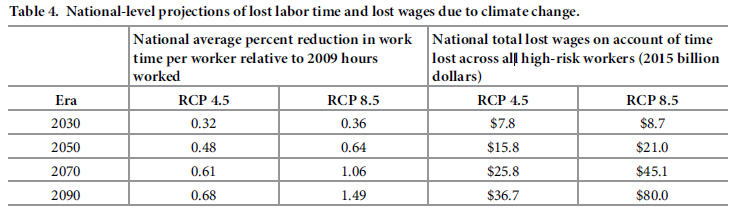
\includegraphics[scale = 0.6]{plots/economic cost.png}
    \caption{Economic cost}
    \label{fig:economiccost}
\end{figure}

Last but not least, it is worth to note that the results of this paper are interpreted as the impact of \textbf{chronic increase in temperature}.
%NEW
%%%%%%%%%%%%%%%%%%%%%%%%%%%%%%%%%%%%%%%%%%%%%
The GZN hazard  model is based on the projections of the climate variable 'daily maximum temperature'. The projected data spans for 20 years. Then, the following statistical processing is used to compute the daily cooling degree days: if the daily number of degrees is higher than $32.2^\circ C$ then the cooling degree days is equal to the number of degrees, and 0 if not. Once the 20-year projected time series of daily cooling degree days is computed, the indicator of the GZN hazard data is calculated as an annual average of the cooling degree days (over all the days within the 20-year period). That indicator will be used afterwards as an input in the impact function to compute the number of minutes of labour productivity loss. Figure \ref{fig:GZL-Hazard} provides a summary of the methodology:

\begin{figure}[h]
    \centering
    %\includegraphics[scale = 0.8]{plots/GZL-Hazard.PNG}
    \caption{Cooling degree days and labour availability}
    \label{fig:GZL-Hazard}
\end{figure}


\subsubsection{Uncertainty around the vulnerability Heat model}

\paragraph{Overview}
The assessment is based on the research performed by Zhang and Shindel, which reviews the uncertainty in the heat risk literature \cite{ZhangAndShindell:2021}. This paper provides context around the uncertainty that exists in the result discussed in previous section, which is mainly explained by the methodology used for the estimation of the impact of temperature on labour productivity. 
\begin{itemize}
    \item \cite{ZhangAndShindell:2021} provides an analysis of the \textbf{differential forecasts} between using the \textbf{GZN method} (as reference to Graff-Zivin and Neidell) documented in \cite{TemperatureAndWork:2021}, versus the WetBulb Globe Temperature methodology (\textbf{WBGT method}) which includes other climate factors in addition to temperature: humidity, wind speed and heat radiation -- figure \ref{fig:WBGT} \footnote{Extracted from \cite{ZhangAndShindell:2021} -- p.4} provides the WBGT detailed approach. 
    \item Another major source of differentiation is that the GZN method focuses on changes in labour allocation decisions while the WBGT method focuses on the physiological impacts of rising temperatures.
\end{itemize}

\begin{figure}[H]
    \centering
    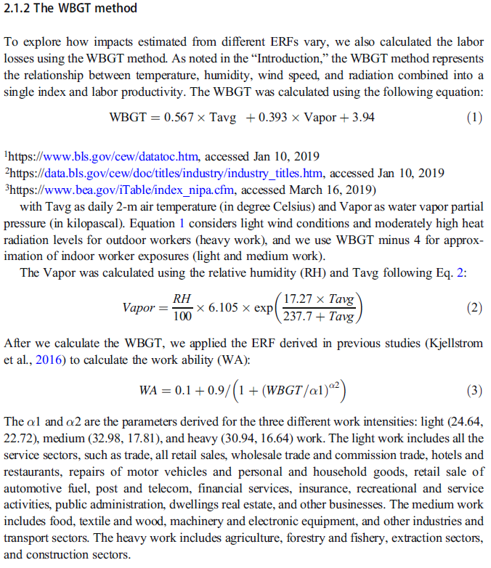
\includegraphics{plots/WBGT.png}
    \caption{WBGT method}
    \label{fig:WBGT}
\end{figure}

The $\alpha1$ and $\alpha2$ are the parameters derived for the three different work intensities: light (24.64, 22.72), medium (32.98, 17.81), and heavy (30.94, 16.64) work.
\begin{itemize}
    \item Light work includes all service sectors, such as trade, all retail sales, wholesale trade and commission trade, hotels and restaurants, repairs of motor vehicles and personal and household goods, retail sale of automotive fuel, post and telecom, financial services, insurance, recreational and service activities, public administration, dwellings real estate, and other businesses.
    \item Medium work includes food, textile and wood, machinery and electronic equipment, and other industries and transport sectors.
    \item Heavy work includes agriculture, forestry and fishery, extraction sectors, and construction sectors. These are the sectors considered in the GZN model methodology, which are the climate exposed sectors. Hence in this study, $\alpha1$ and $\alpha2$ of the heavy work intensity are applied $(30.94, 16.64)$.
\end{itemize}



Note that there are differences in the functional forms applied in the original GZN method \cite{TemperatureAndTheAllocationofTime:2014} and the approach presented in \cite{TemperatureAndWork:2021}, with original GZN method using one linear regression with dummy variables for temperature buckets, while \cite{TemperatureAndWork:2021} uses multiple linear regressions with one variable reflecting the breach of the maximum temperature around anchor points (less than $70^\circ F$, $90^\circ F$, $90^\circ F$ and above). The WBGT methodology uses a non-linear function to relate labour loss to the WBGT consolidated measure.   

Figure \ref{fig:CostsByRCP} \footnote{Extracted from \cite{ZhangAndShindell:2021} -- p.11} provides the forecasts of labour lost millions of 2016 USD (constant USD value). Most notably the original GZN produces more optimistic forecasts of the cost of labour lost (lower) than the WBGT method. Note that RCP8.5\footnote{The Intergovernmental Panel on Climate Chance modelling are based on representative concentration pathways (RCPs), which represent different emissions projections under basic, plausible economic and social assumptions, while staying within physical constraints. RPCs are constructed by back-calculating the amount of emissions that would result in a given amount of radiative forcing (which is the difference between solar radiation (energy) absorbed by the Earth and energy radiated back into the space) that would then result in a given amount of warming} refers to the scenario of high emissions and RCP4.5 refers to the scenario of moderate emissions.

\begin{figure}[h]
    \centering
    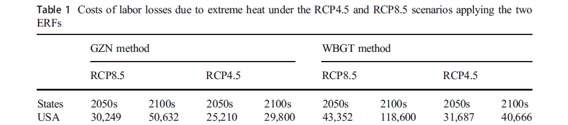
\includegraphics{plots/CostsByRCP.png}
    \caption{Costs By RCP under GLZ method versus WBGT method}
    \label{fig:CostsByRCP}
\end{figure}



\paragraph{Detailed approach: vulnerability around GLZ model}

There are 2 identified areas where uncertainty in the forecasts in \cite{TemperatureAndWork:2021} paper: the economic cycle and the model parameter uncertainty.
\newline
The \textbf{economic cycle} is one area where uncertainty exists in the forecasts. 
The paper shows that labour allocation decisions are sensitive to where in the economic cycle the US is; during a recession there does not appear to be a relationship between labour allocation and temperature. In order to measure the uncertainty explained by the economic cycle, one might consider the probability of a recession as a Bernoulli random variable with a probability p. Based on this there are two possibly approaches. A first approach is a Monte-Carlo like approach where one can randomly sample the 1, 0 value whether a recession occurs at each period on a time path. A second approach would be to use the expected value of the probability of the recession and estimate the impact as: 
\begin{equation}
    \label{Eq:economiccycle}
    	Forecasted \ Minutes \ Lost = p \times 0 + (1-p) \times EV(X)
\end{equation}
Where $X$ is the variable that refers to Minutes Lost during normal economic cycle
The second approach is attractive in its simplicity and ensuring the model does not lose its focus. 
One concern is that the probability of recession, in reality, may be related to the realisation of climate related risks. Hence, there might be a over/under estimation of the probability unless the impact of the climate risk is also considered. Historical model estimated recession probabilities can be sourced from \cite{SmoothedU.S.RecessionProbabilities:2022}. However, we did not go further in the measurement of the uncertainty explained by the economic cycle because it requires us to focus on the modelling of another parameter ($p$, the probability of the recession to occur), which is not the purpose of this work. 

%%%%%%%%%%%%%%%%%%%%%%%%%%%%%%%%%%%%%%%%%%%%
% to add in the references: https://github.com/os-climate/physrisk/blob/main/methodology/PhysicalRiskMethodologyBibliography.bib
%%%%%%%%%%%%%%%%%%%%%%%%%%%%%%%%%%%%%%%%%%%%
%@article{SmoothedU.S.RecessionProbabilities:2022,
%  title={Smoothed U.S. Recession Probabilities},
%  author={Jeremy Piger},
%  publisher={University of Oregon}
%  year={2022},
%}
Instead, we focus on the \textbf{model parameter uncertainty approach}. In \cite{ZhangAndShindell:2021}, there is a linear relationship between temperature and work minutes lost ($\beta$),and a constraint is applied to ensure that total time allocation sums to 24 hours, which returns a non-linear regression model at the end. Given that the main coefficient of interest is denoted $\beta$, an inference is applied assuming that $\beta$ follows a $Student-T$ distribution: 
\begin{equation}
 \label{Eq:uncertaintyStudentT}   
 d\beta \sim T(\beta, SE, N-K)
\end{equation}
Where $SE$ is the Standard Error of the coefficient and $(N-K)$ is the number of degrees of freedom, $N$ is the number of observations and $K$ is the number of model parameters. Hence, one can estimate the coefficients of the confidence interval (CI) at a given level of confidence $CI\%$: 
\begin{equation}
 \label{Eq:CIStudent}   
 d\beta_{CI\%} = \beta \pm T(p) \times SE
\end{equation}
Where $T(p)$ donates the probability density function (pdf) of the student $T$ distribution with probability $p$ which corresponds to the $CI\%$, the standard error $SE = 2.23 \ min$ and $\beta =  - 4.68$.

%%%%%%%%%%%%%%%%%%%%%%%%%%%%%%%%%%%
%START HERE
%%%%%%%%%%%%%%%%%%%%%%%%%%%%%%%%%%%

Figure \ref{fig:GZL-Vulnerability} shows the uncertainly around the GZN vulnerability model, based on the assumptions above, at $95\%$ confidence level\footnote{In order to compute the figure, N is taken from the paper \cite{TemperatureAndWork:2021}: N 11,732, and K is assumed to be 0 as it is very small relatively to N. One could do further researches to check the exact number of K, but that will not impact the results. K includes the number of control variables which provide information on demographic data -- age, gender, education, employment status, income, etc. -- and climate variables such as level of precipitation and snow.}.
\begin{figure}[h]
    \centering
    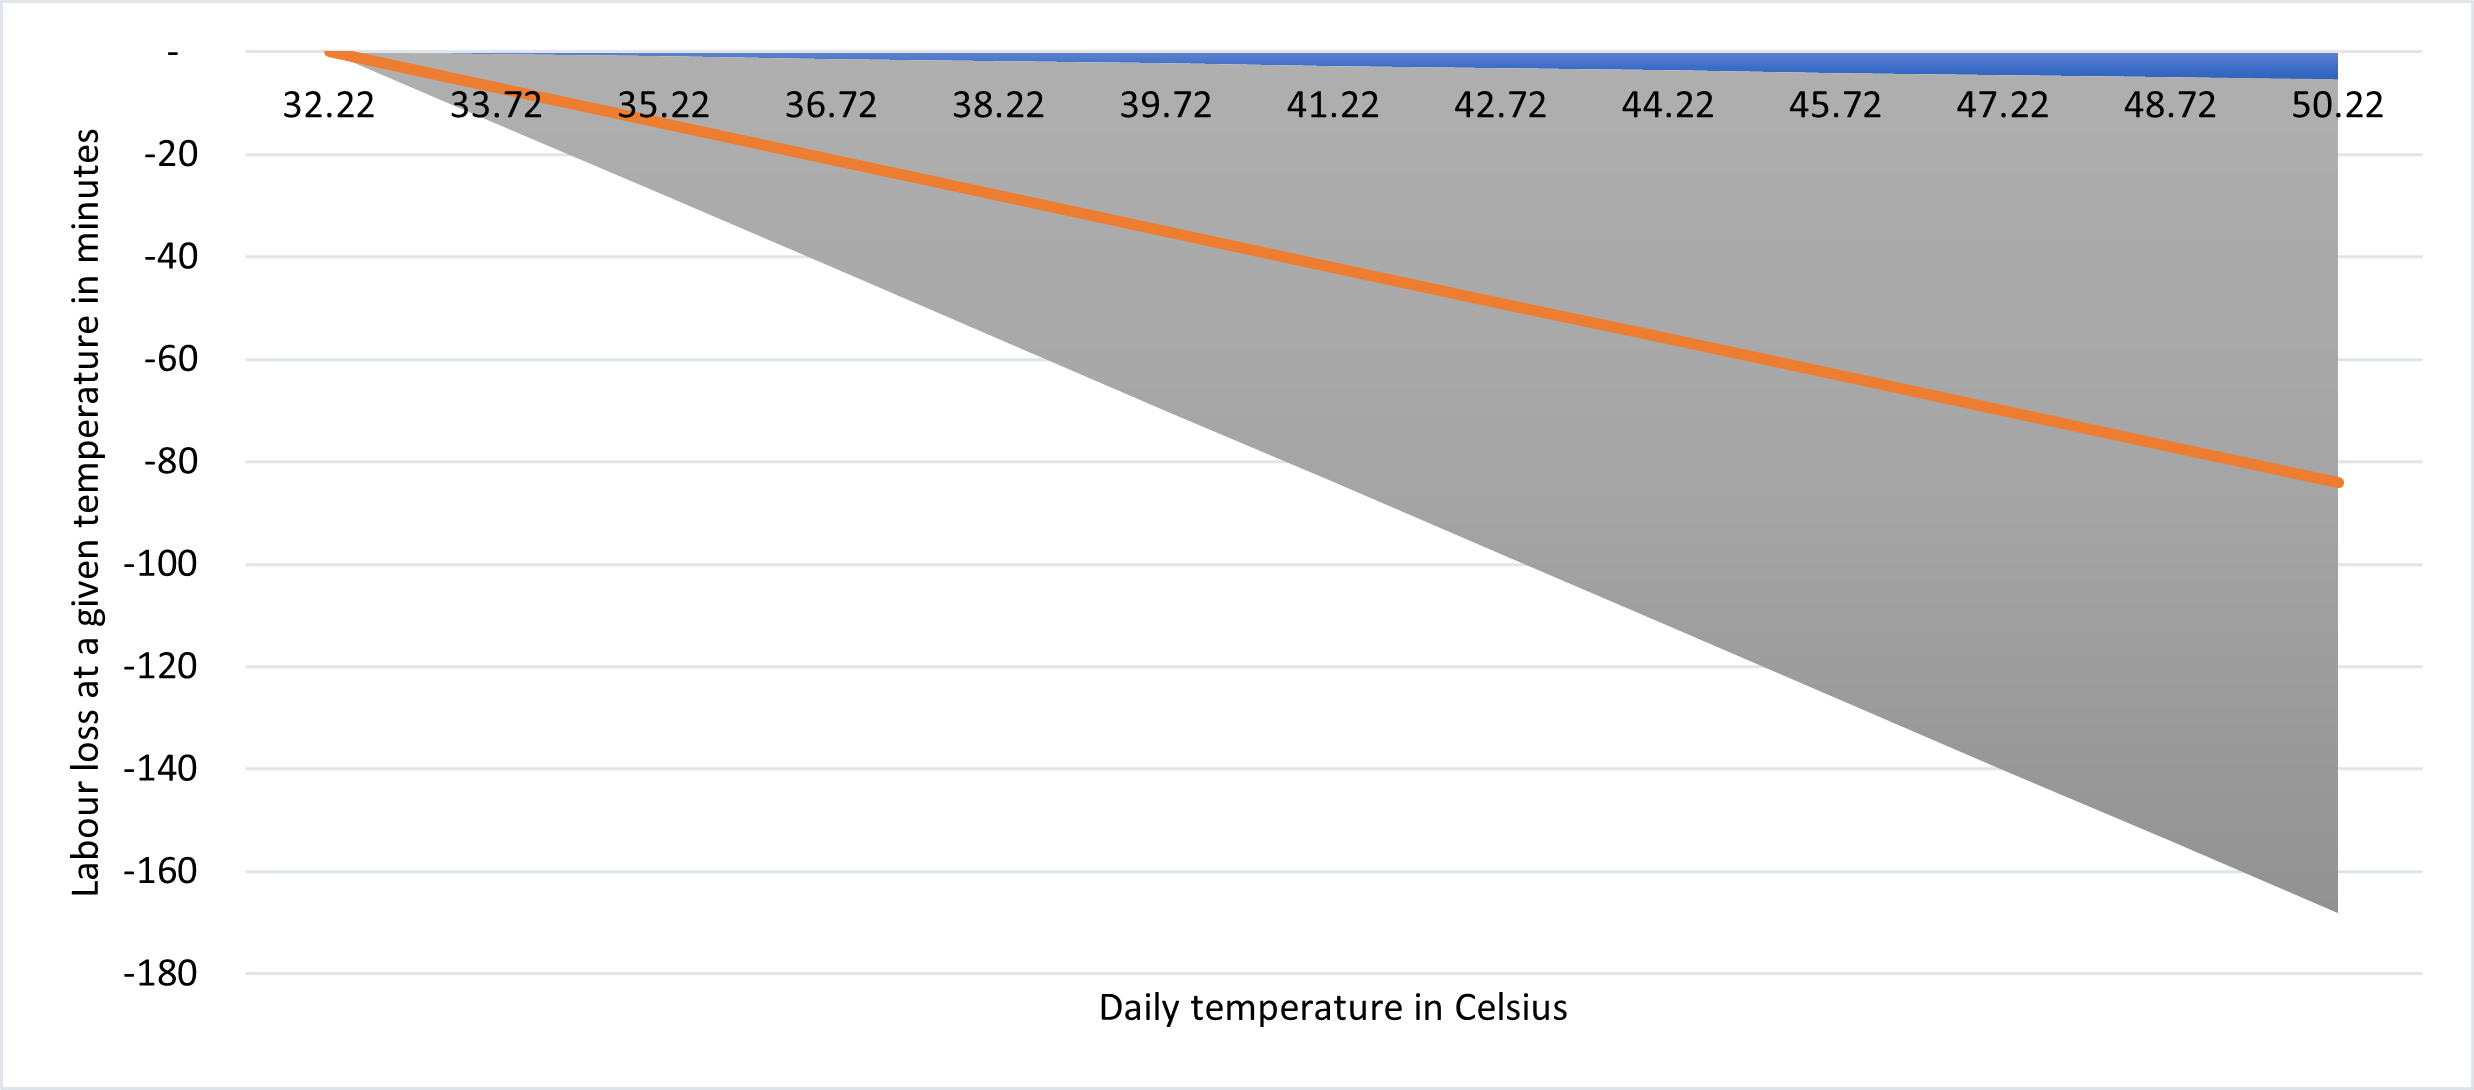
\includegraphics[scale = 0.8]{plots/GZL-Vulnerability.png}
    \caption{Estimate of daily minutes of labour loss}
    \label{fig:GZL-Vulnerability}
\end{figure}


As the degrees of freedom increases, the t distributions converge to the standard normal. Therefore, for simplicity reasons in the context of this work, it is assumed that that the daily labour productivity impact $\beta$ can be measured as:
\begin{equation}
    \label{Eq:uncertainty1}
    	\beta \sim \mathcal{N}(m,\,SE^{2})\,\ where \ m = 4.68 \ min \ and \ SE = 2.23 \ min
\end{equation}


As an example, consider an $1.5^\circ C$ degree day increase in the temperature. We can then multiply through the normal distribution as shown below: 

%The buckets of the daily maximum temperature above $32.2^\circ C$  are defined as an incremental increase of $1.5^\circ %C$, starting from $0^\circ C$ to $18^\circ C$: $\begin{pmatrix} 0 & 1.5 & 3 & ... & 18 \end{pmatrix}$. For a $1.5^\circ %C$ daily temperature increase, the uncertainty around the daily labour productivity impact is given by the following %normal distribution:
\begin{equation}
    \label{Eq:uncertainty2}
    1.5 \times \beta \sim \mathcal{N}(1.5 \times \beta,\, (1.5 \times SE)^{2})\, 
\end{equation}

This can be generalised for a degree day increase of x using the following distribution: 


\begin{equation}
    \label{Eq:uncertainty3}
    x \times \beta \sim \mathcal{N}(x \times \beta,\, (x \times SE)^{2})\, 
\end{equation}
For example, there is 1\% chance that the lost labour productivity exceeds $29.6$ minutes per day if the maximum daily temperature exceeds at $32.2^\circ C$ by $3^\circ C$. This number is computed as $\mathcal{N}^{-1} (m',SE'^2)(1\%)$ where $m'= 3 \times m = -14.013 \ min$ and $SE'= 3 \times SE = 6.69 \ min$. The $99\%CI$ of the lost labour productivity per day if the maximum daily temperature exceeds at $32.2^\circ C$ by $3^\circ C$ is $[+1.6 \ min, -29.6 \ min]$.

%Adding point regarding impact as a percentage of total labour 


The estimated loss of labour time is then transformed into a percentage estimate:

\begin{equation}
    \label{Eq:uncertainty3}
    Estimated \ loss \ of \ labour \ time \ (\%)=  \frac{Labour \ lost}{Total \ minutes \ worked \ in \ a \  year}\
\end{equation}
For this the figures reported by the Organisation for Economic Co-operation and Development (OECD) are used, specifically the 2021 estimate for the United States of America. This is to ensure the alignment with the region where the labour parameters are estimated in. Buckets of labour lost are defined within the range of no impact to 100\%, with estimated marginal probabilities for each bucket returned.


The main weakness of the Temperature and Work article (which is more likely to be close to the original GZN method than to the WBGT method) is that it does not take into account of higher levels of optimism in the original GZN method which was noted in figure \ref{fig:CostsByRCP}. Hence, the results might be underestimating the actual impact. The next paragraph explores the vulnerability model around the WBGT method and its uncertainty.

\paragraph{Detailed approach: vulnerability around WBGT model}

%NEW
%%%%%%%%%%%%%%%%%%%%%%%%%%%%%%%%%%%%%%%%%%%%%
The WBGT hazard model, as show in figure \ref{fig:WBGT-Hazard}, is based on the projections of the climate variables 'daily temperature' and 'daily humidity'. The projected data spans for 20 years. Then, the computations provided in figure \ref{fig:WBGT} are used to compute the daily WBGT, which is considered as the indicator of the WBGT hazard data that will be afterwards considered as an input in the impact function to get the daily Work Ability (WA) projections over the 20-year period. Finally, the impact deriving from the WBGT model is computed as the annual average of the daily projected WA.
\begin{figure}[h]
    \centering
    %\includegraphics[scale = 0.8]{plots/WBGT-Hazard.PNG}
    \caption{WBGT and labour availability}
    \label{fig:WBGT-Hazard}
\end{figure}
Note that another indicator deriving from the WBGT hazard model is the Work Loss (WL), which is computed as $WL = 1 - WA$. It is another way to do the assessment but leads to same results. 
\newline
The aggregation of the outputs of the GZN vulnerability model (minutes of productivity labour loss) and the WBGT vulnerability model (WA), returns the effective number of working hours, which represents a way to measure the uncertainty around the GZN vulnerability model. Figure \ref{fig:Aggregation} provides the aggregation process and results:
\begin{figure}[h]
    \centering
    %\includegraphics[scale = 0.8]{plots/Aggregated Hazard WBGT GZN.PNG}
    \caption{Aggregation of GZN model and WBGT model}
    \label{fig:Aggregation}
\end{figure}
If the WL was used instead of the WA, then it will be multiplied by the hours worked derived from the GZN model to get the annual total labor loss due to heat.

Given the modelling assumptions around the parameters used to compute the WA in the WBGT model, it is important to measure the uncertainty around these parameters, $\alpha1$ and $\alpha2$, which depend on the work intensities. 

The source paper provides the parameters $\alpha1$ and $\alpha2$ for three different work intensities low, medium and high with industries mapped to each intensity. These categories are broad and do not account for variance within and industry and between industries in the same category. To account for this uncertainty the WBGT approach was adjusted to include uncertainty around the industry.

Consider an asset which is market as in a high risk sector. We assume that the work ability is uniformly distributed with a mean equal to the $WA_H$ and a floor (a) and ceiling (b) equidistant from the mean. We assume that the floor a is halfway between $WA_H$ and $WA_M$. So a and b can be estimated based on the below formulae: 

\begin{equation}
    \label{Eq:WBGT_Floor}
     a = WA_H - \frac{WA_H - WA_M}{2}\,
\end{equation}

\begin{equation}
    \label{Eq:WBGT_Ceil}
     b = WA_H + \frac{WA_H - WA_M}{2}\,
\end{equation}

And the WBGT work ability can be represented based on the below formula: 

\begin{equation}
    \label{Eq:WBGT_Uniform}
     WA \sim \mathcal{U}(a ,b)\, 
\end{equation}
 
With this we can estimate the variance of the WBGT work ability using the standard formula for the variance of a Uniform distribution:

\begin{equation}
    \label{Eq:WBGT_Variance}
     Var(WBGT) = \frac{(a-b)^2}{ 12}
\end{equation}

In order to get to a final work ability we multiple the output of the GZN model by the ouput of the WBGT model.

\begin{equation}
    \label{Eq:Final_Mean_WA}
     Effective Work = (1- Estimated \ loss \ of \ labour \ time ) \times WA_H
\end{equation}

As we have uncertainty both for the GZN component as well as the WBGT component we need to estimate a joint variance. We assume that the epistemic uncertainty in the GZN model is uncorrelated with the variance in the sector uncertainty of the work ability measure. To estimate the variance of the product of both the GZN and WBGT components we using the following formula:

\begin{equation}
\begin{aligned}
    \label{Eq:Var_Joint}
     Var(EffectiveWork) = (1- Estimated \ loss \ of \ labour \ time )^2 \times Var(WBGT) + \\
      WA_H^2 \times Var(GZN) +  var(WBGT) \times Var(GZN) 
      \end{aligned}
\end{equation}

To get the final impact we assume that the product of the two variables are normally distributed. The final work ability distribution can be represented as below:

\begin{equation}
\begin{aligned}
    \label{Eq:Final_Result_Heat}
     N(EffectiveWork, Var(Effective Work))
      \end{aligned}
\end{equation}

\clearpage
\printglossaries
\clearpage
%%%%%%%%%%%%%%%%%%%%%%%%%%%%%%%%%%%%%%%%%%%%%%%%%%%%%%%%%%%%%%%
\bibliography{Physical Risk Methodology Bibliography}
%%%%%%%%%%%%%%%%%%%%%%%%%%%%%%%%%%%%%%%%%%%%%%%%%%%%%%%%%%%%%%%

%\bibliographystyle{plain}
\bibliographystyle{acm}
%\bibliographystyle{agsm}



\end{document}
